\documentclass[draftclsnofoot,10pt,onecolumn]{IEEEtran}
\usepackage[T1]{fontenc}
\usepackage[utf8]{inputenc}
\usepackage[letterpaper, margin=0.75in]{geometry}
\usepackage[en-US]{datetime2}
\usepackage{xcolor}
\usepackage{pdfpages}
\usepackage{hyperref}
\usepackage{longtable}
\usepackage{listings}
\title{Programming For Underrepresented High School Students - Project Archive}
\author{Isak Foshay, Rebecca Croysdale, Cristian Mann, Roy Simons}
\begin{document}
\maketitle
\begin{center} Spring Term: \today \end{center}
\begin{center} Team: CS67 aka: "Get Good, Kids!"\end{center}

\newpage
\tableofcontents

\newpage
\section{Forward: Release Notes}
Features that could be implemented in the future:
\begin{itemize}
\item{Lesson curriculum: A set of lessons that can be started with no coding experience, and ends with machine learning. Implemented in Blockly and stored in the default database.}
\item{Re-orderable lessons: The teacher should be able to change the order of the lessons at any time. Currently, each new lesson is put at the end of the list of lessons when they are made.}
\item{Lesson modules: A teacher should be able to group lessons together in modules. The modules should be hidden from the students by default until the teacher publishes them.}
\item{Password recovery: A user should be able to recover their password via email if they forgot it.}
\item{Student made lessons. A student should be able to make lessons for other students to try. These lessons should not affect the students grade, and each student should have a maximum number of lessons that they can make.}
\item{Add input to lessons. When making a grading script, the teacher should be able to sample the student's code with different input for grading. For example, in the sort lesson, the teacher could send different lists as input.}
\item{Teacher's student view. A teacher should have a button they can press to switch to student view. This mode would be similar to canvas's student view mode.}
\end{itemize}

\section{Introduction to the project}
\subsection{Who requested it?} % seems like the same question as below
Our client Shashi Jain from Intel, inc.
\subsection{Why was it requested?}
At a Native American high school career fair, Shashi Jain experienced that the students of the high school did not expect a company like Intel to be there. The student barely had the idea that they had the option pursue an education/career in computer science, which was a trigger to create a project to give high school students with limited access to internet and tech, the chance to learn computer science concepts.
\subsection{What is its importance?}
The importance of the project is to give high school students with limited access to internet and tech, the opportunity to learn more about computer science. Knowing more about computer science hopefully leads to these students realizing that they can pursue an education and career in a computer science field.
\subsection{Who are the members of your team?}
Isak Foshay, Rebecca Croysdale, Cristian Mann and Roy Simons
\subsection{What were their roles?}
Isak Foshay did project management, grading implementation, and setup script creation.
Rebecca Croysdale created the majority the UI including routing between pages, made several large changes to the database, implemented conditional viewing based on logged in user, and created small UI components for better modularity.
Cristian Mann initialized the SQLite database and created much of the API server routing that interacts with the database and the React server, as well as security in the form of encrypting sensitive data for privacy, using JSON web tokens to authenticate users, and create timed one-time passwords for teacher registration to ensure authority.
Roy Simons did the user interface setup/design, hamburger menu, user interface look improvement and tutorials/explanation on how to use the application and do/create lessons.
\subsection{What was the role of the client(s)?} %  (I.e., did they supervise only, or did they participate in doing development)}
For most of the project our client, Shashi Jain, supervised the progress, and came with new ideas and expectations for the project. The client was open for new ideas for the project, but had certain expectations for the project.
\subsection{How did the changes in spring term affect your deliverables?}
We decided to make the app more teacher tool based rather than creating lessons, because we would not be able to test the lessons with users. We implemented two different user types, as well as lesson creation for the teacher user type. We also implemented a one time password with a QR code access, ensuring that students could not create a teacher account.

%\subsection{How do you recommend the next team use this final documentation to pick up where you left off?} %(Refer readers to Appendix 3—that’s where you’ll write up the remaining work to do).

\clearpage
\section{Requirements document}
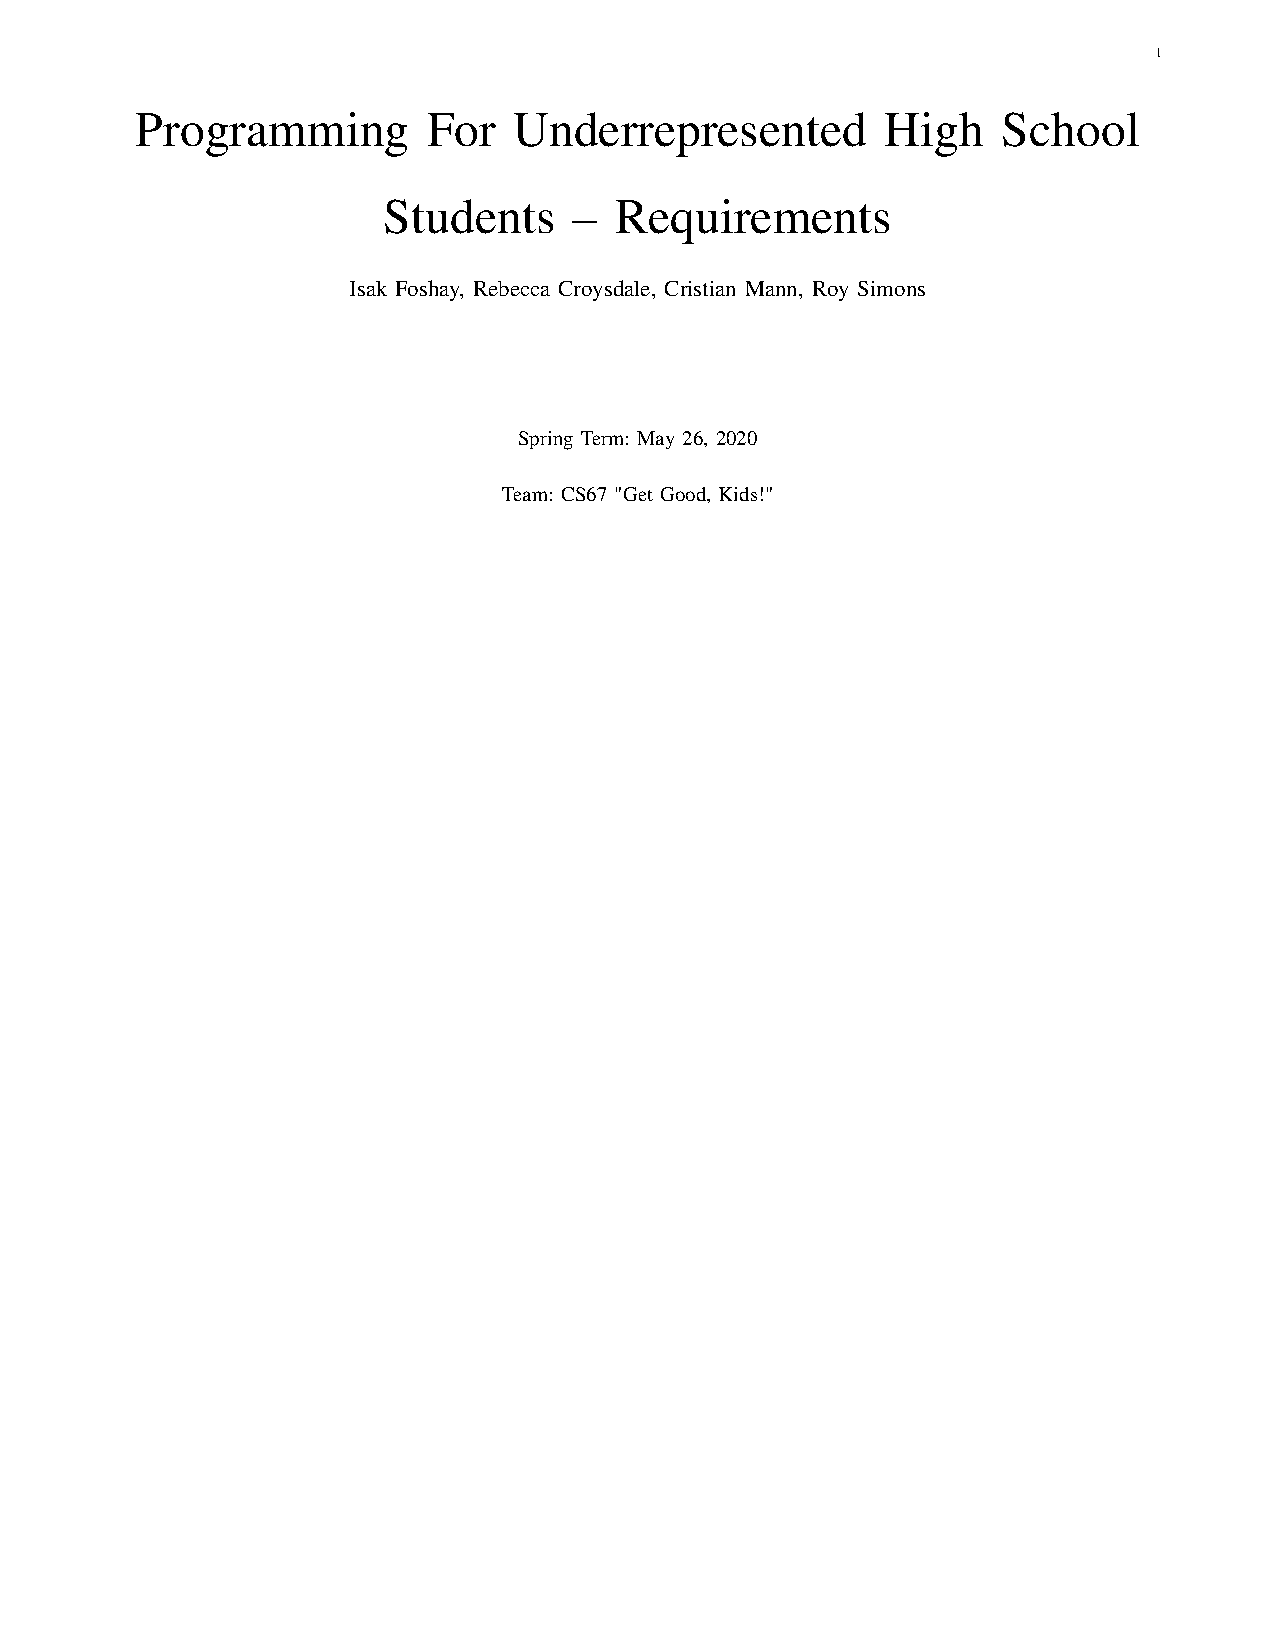
\includepdf[pages=-,pagecommand={},width=1.18\textwidth]{Requirements_2_0.pdf}

\clearpage
\section{Design document}
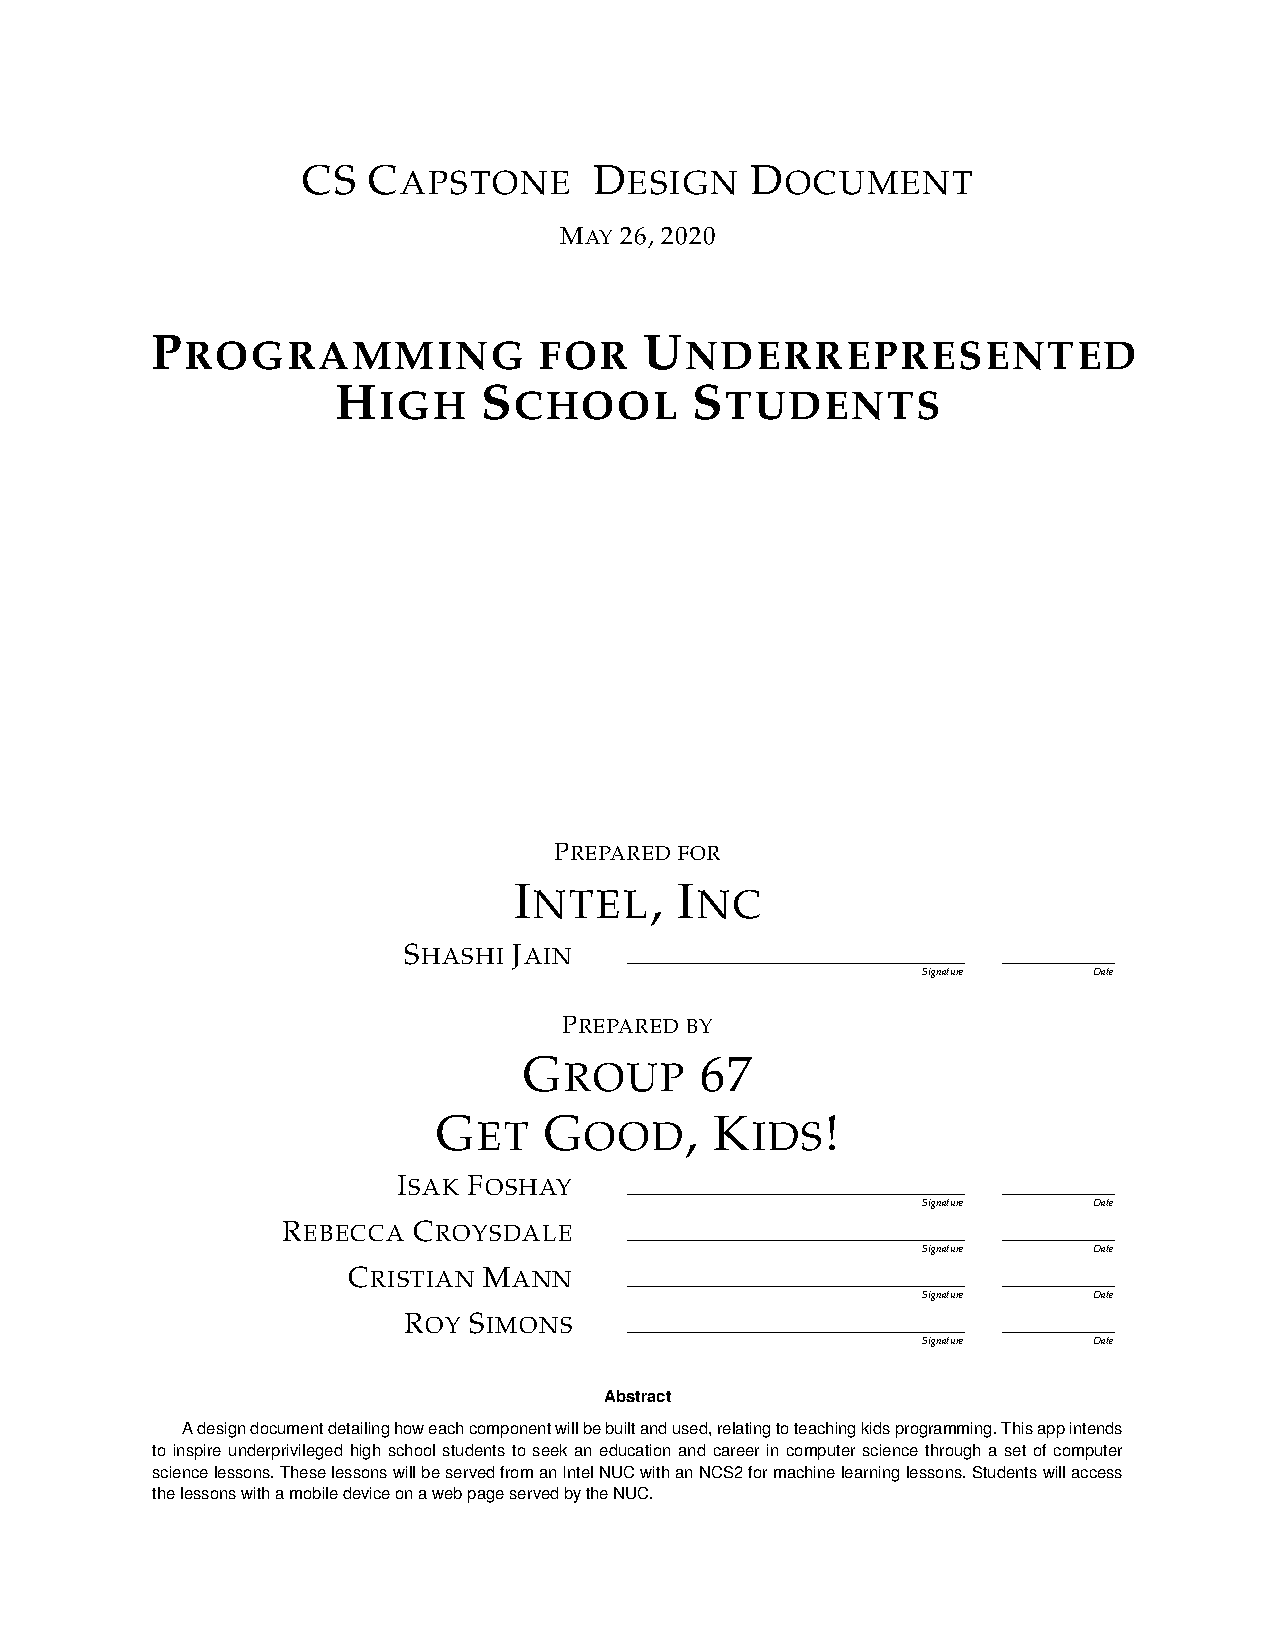
\includepdf[pages=-,pagecommand={},width=1.18\textwidth]{Design_Document_2_0.pdf}

\clearpage
\section{Tech reviews}
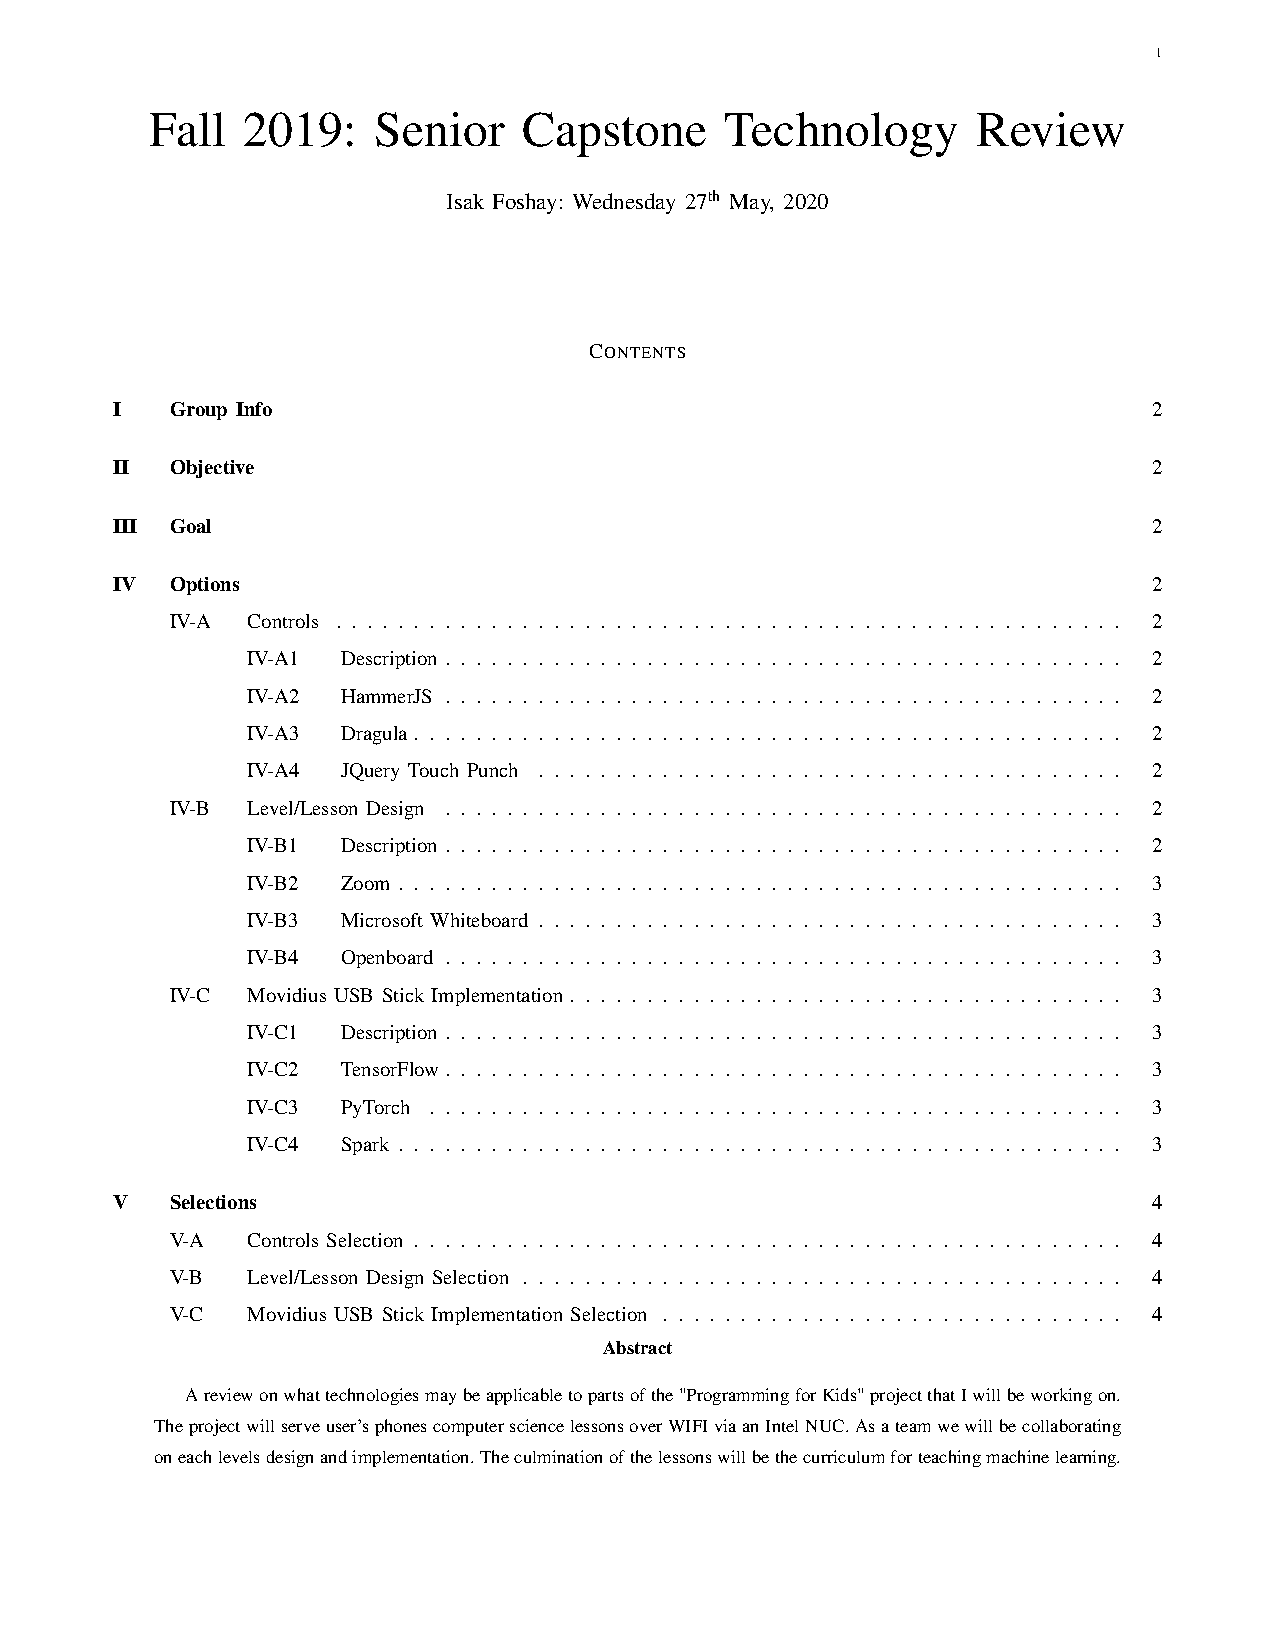
\includepdf[pages=-,pagecommand={},width=1.18\textwidth]{Technology_Review_Isak.pdf}
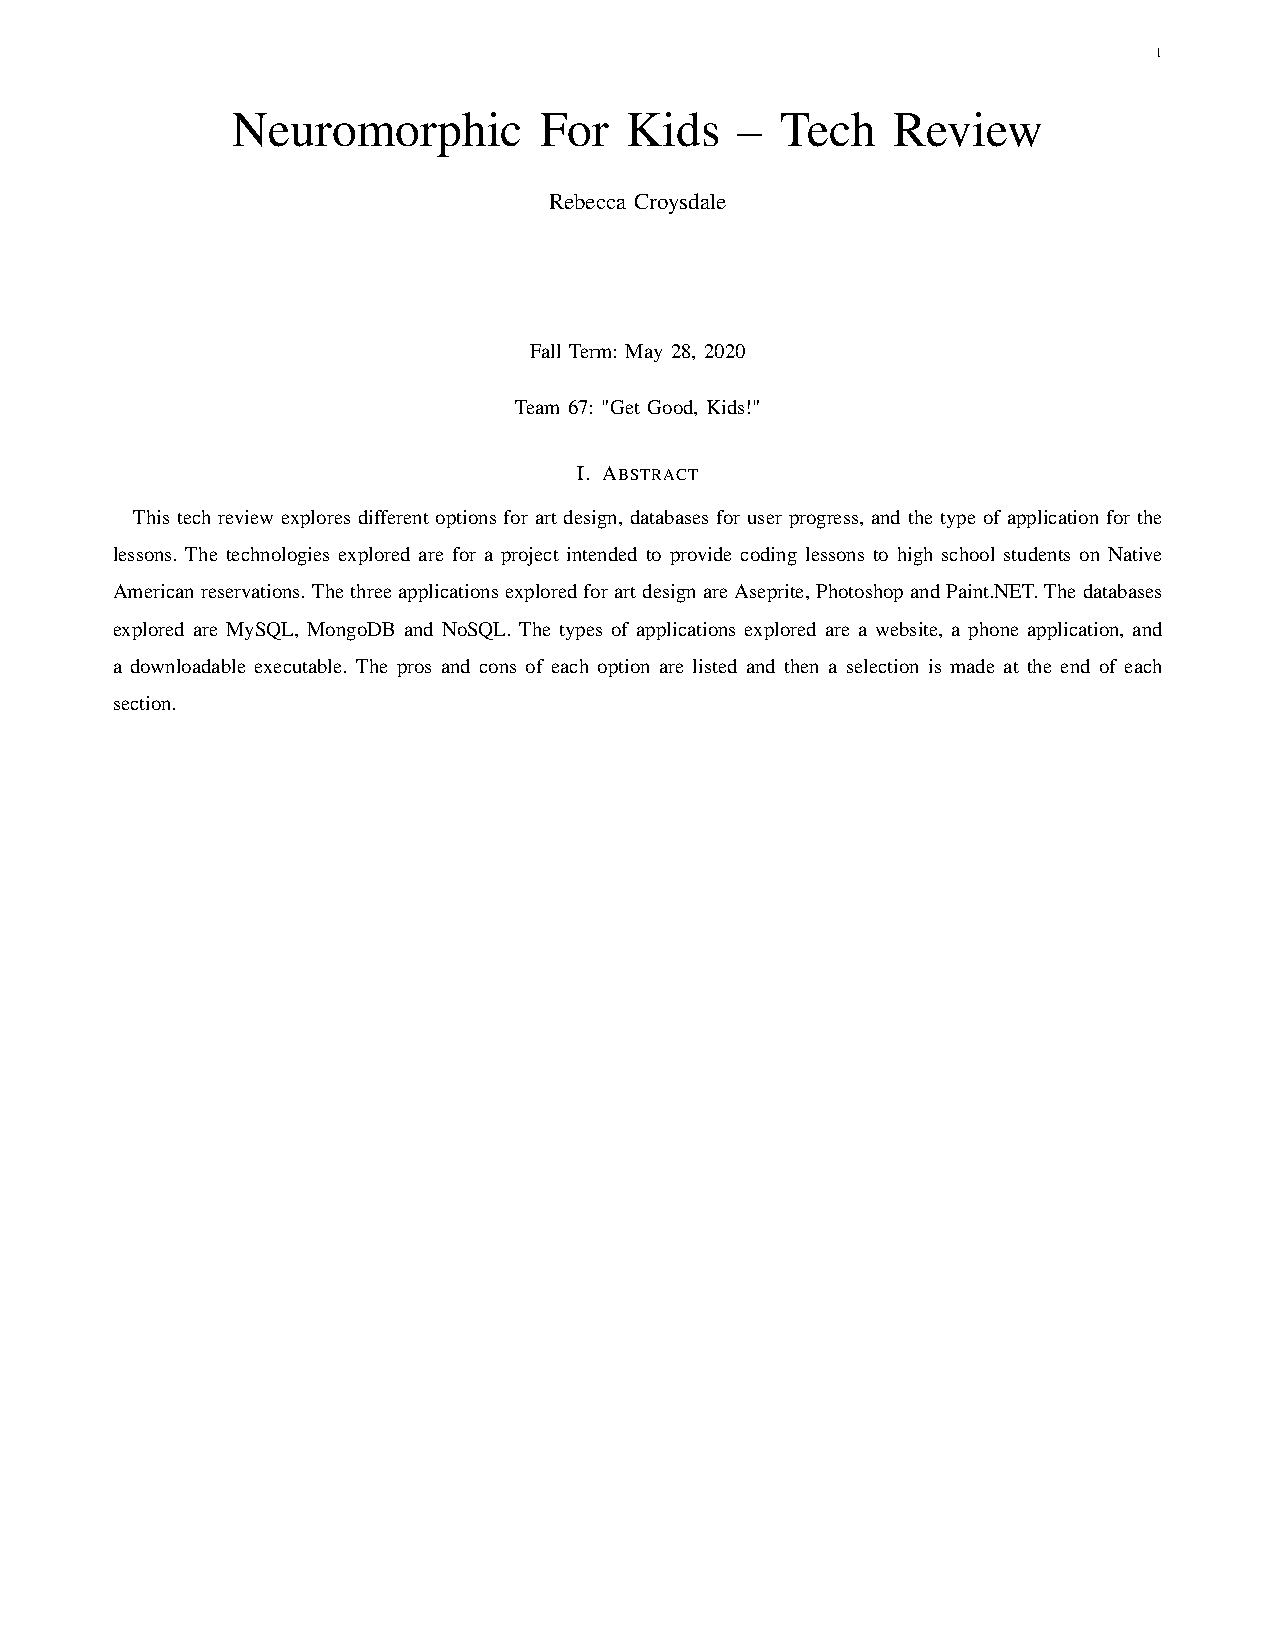
\includepdf[pages=-,pagecommand={},width=1.18\textwidth]{Tech_Review_Rebecca.pdf}
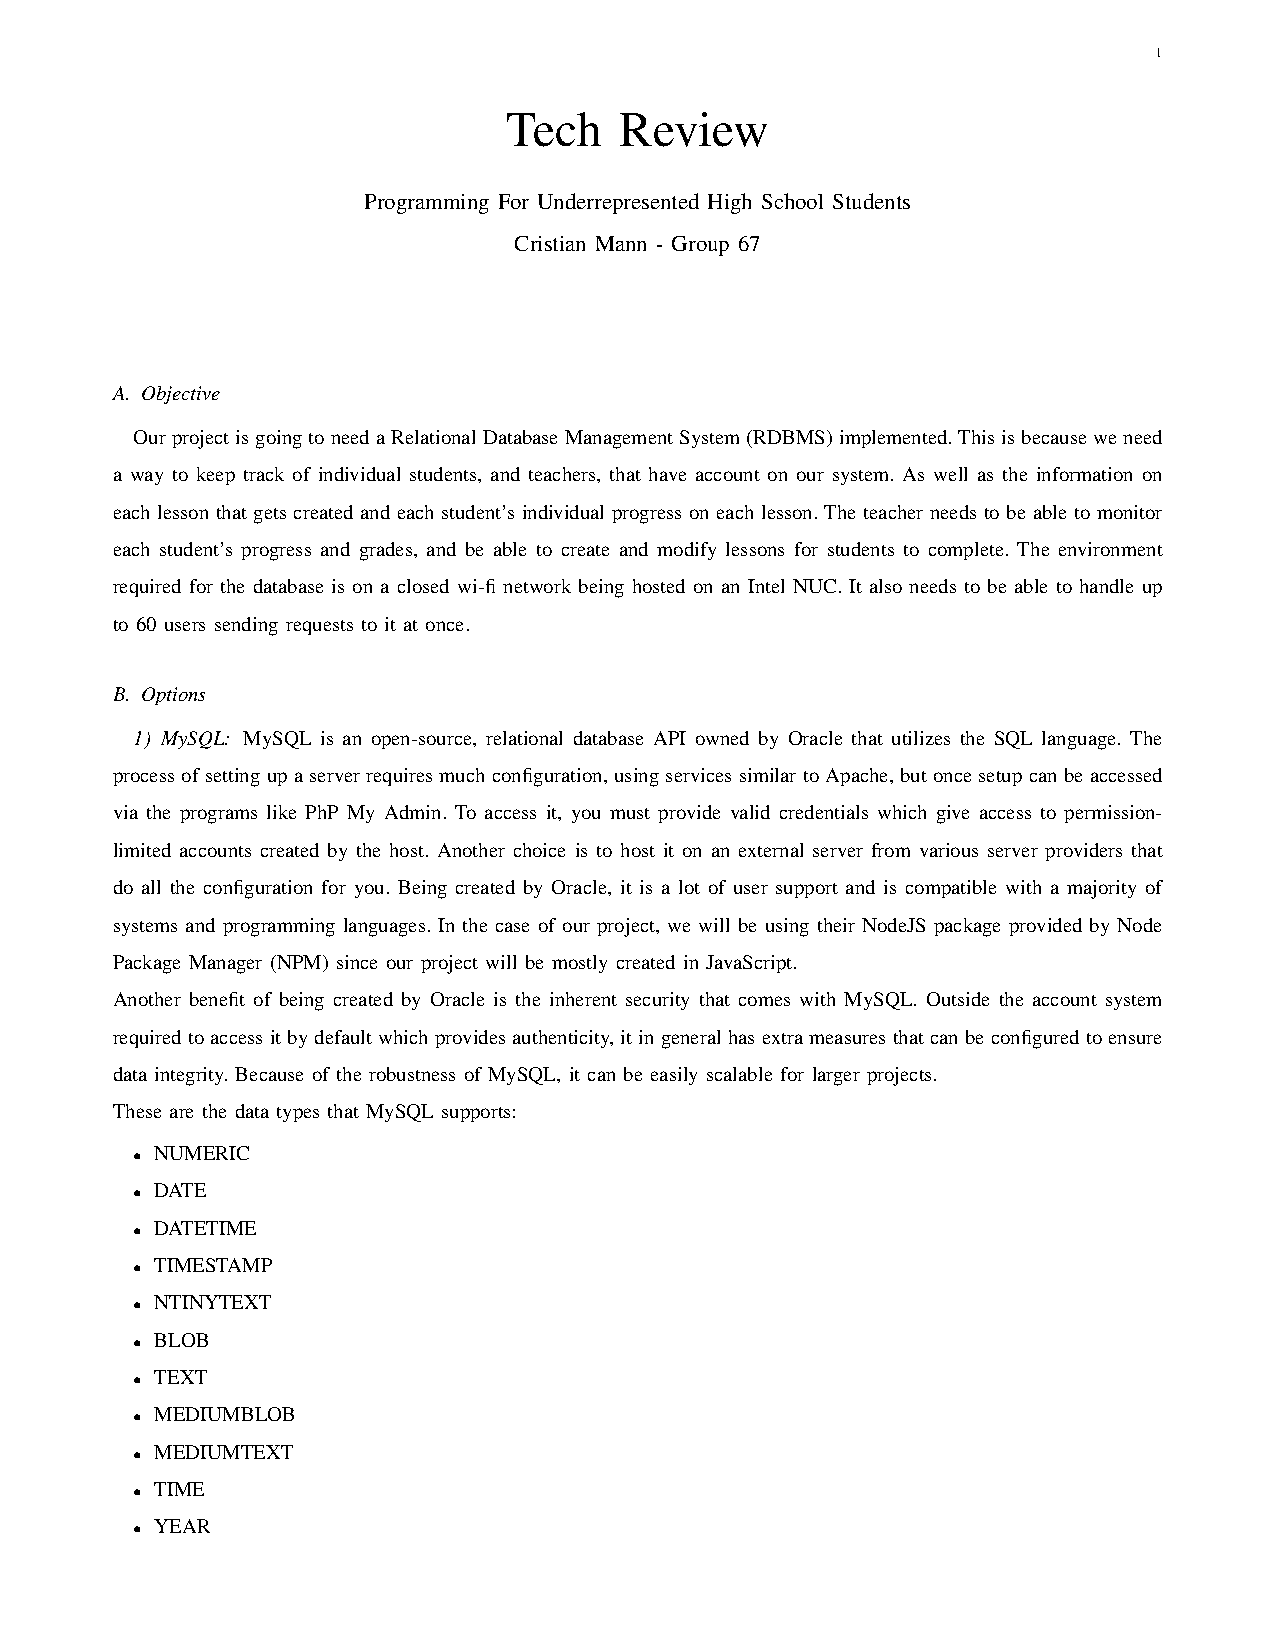
\includepdf[pages=-,pagecommand={},width=1.18\textwidth]{Tech_Review_Cristian.pdf}
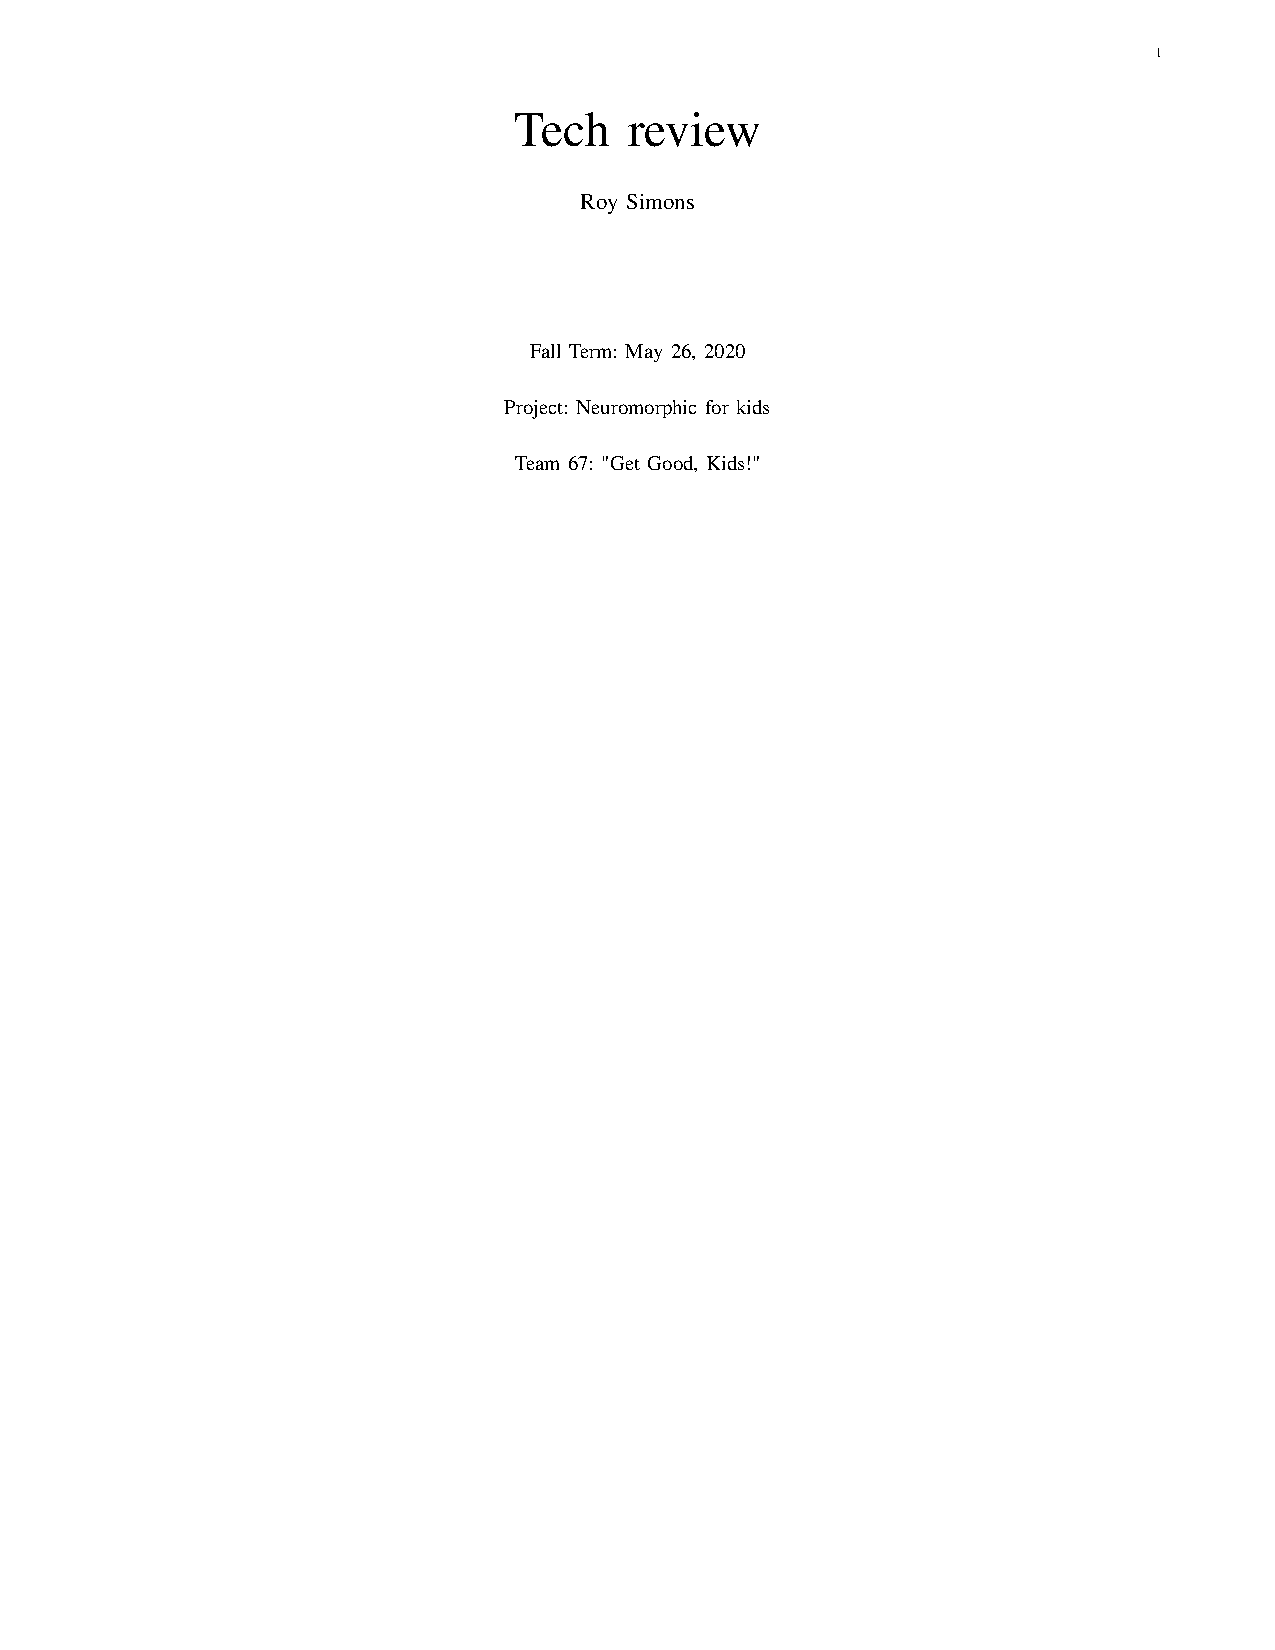
\includepdf[pages=-,pagecommand={},width=1.18\textwidth]{Tech_Review_Roy.pdf}
%\clearpage
\section{Weekly blogs}
\subsection{Isak Foshay Weekly blogs}
\begin{tabular}{p{0.1\linewidth}p{0.3\linewidth}p{0.3\linewidth}p{0.2\linewidth}}
        \hline
            \textbf{Week}
             & \textbf{Positives}
             & \textbf{Deltas}
             & \textbf{Actions}\\
             \hline
             Week 1
             & ------
             & ------
             & ------\\
             \hline
             Week 2
             & ------
             & ------
             & ------\\
             \hline
             Week 3
             & Started working on the requirements document and had a meeting with the client
             & Not getting to talk with the client until this week. Loose constraints on what is being asked for
             & We will finish the requirements document and attempt to solidify what our project is going to look like\\
            \hline
             Week 4
             & We fleshed out more of the requirements document
             & We haven't heard from the client in a while
             & We think we will make a game that uses lessons to unlock code blocks in order to solve challenges\\
            \hline
             Week 5
             & We have more of a concrete vision of what the project is going to look like. We will be using Scratch elements in the final product. Shashi will be sending us some hardware (AI stick and NUC).
             & The client not having a concrete vision results in added difficulties with doing all of the documentation for the class before we have started working on the project.
             & We will experiment with having the lessons packaged as a story based game that integrates Native American culture.\\
            \hline
             Week 6
             & We now finally know that the project will be Javascript based and served off of an Intel NUC.
             & We did not have a concrete view of what our project was going to look like until 2:30pm on Friday with 10.5 hours to finish the tech review.
             & Our plan is to begin to flesh out how we are supposed to make the lessons into a game when it is on the phone's limited screen space.\\
            \hline
             Week 7
             & We decided to pursue a card game based project in order to promote an enjoyable user experience on the phone.
             & We are not sure what a design document entails for our project.
             & We will finish the design document soon and send a copy to Shashi for his opinions.\\
            \hline
             Week 8
             & We have a better understanding of what the Design Document should look like as well as what our project will be.
             & We ran into problems understanding what the Design Document should look like and convey.
             & We will finish the Design Document tomorrow\\
            \hline
             Week 9
             & Taking a break for thanksgiving gave the Team a time to refresh and refocus for the rest of the term.
             & No problems this week.
             & We will regroup on what needs to be done once school resumes.\\
            \hline
             Week 10
             & We are excited to begin working on the project this coming term.
             & We haven't received grades yet for the Design Document which is a little unsettling.
             & We will wait for Shashi to give us feedback on our documents.\\
            \hline
             
        \end{tabular}
        \newpage
        \begin{tabular}{p{0.1\linewidth}p{0.3\linewidth}p{0.3\linewidth}p{0.2\linewidth}}
        \hline
            \textbf{Week}
             & \textbf{Positives}
             & \textbf{Deltas}
             & \textbf{Actions}\\
            \hline
             Week 11
             & We have set up a meeting time for our client meetings to happen.
             & no problems yet.
             & I will work to get the nuc serving a website to access via the local network.\\
            \hline
             Week 12
             & Found blocky which will make turning block based code into a grade able format easier. looking in to how to make custom blocks in order to implement machine learning lessons.
             & Not completely sure how to sandbox python properly for grading.
             & potentially contact someone in the cs department at OSU to ask about making grading scripts.\\
            \hline
             Week 13
             & ---
             & ---
             & ---\\
            \hline
             Week 14
             & ---
             & ---
             & ---\\
             \hline
             Week 15
             & Getting docker to work with combining grading scripts plus user generated code
             & Blockly is a bit difficult to work with
             & Make creating grading scripts more streamlined.\\
             \hline
             Week 16
             & code generated from blockly passed to proxy server for grading. almost finished making the grading scripts
             & blockly outputs 2 space tabs and I need 4 space tabs
             & finish making grading scripts and grading process.\\
             \hline
             Week 17
             & ---
             & ---
             & ---\\
             \hline
             Week 18
             & ---
             & ---
             & ---\\
             \hline
             Week 19
             & ---
             & ---
             & ---\\
             \hline
             Week 20
             & sent email with tech requirements to bill (Online capstone instructor). 
             & demo video will be hard to make with everyone in quarantine.
             &  make demo video from people's homes instead of meeting up. \\
            \hline
            \end{tabular}
            \newpage
\subsection{Rebecca Croysdale Weekly blogs}        \begin{longtable}{p{0.1\linewidth}p{0.3\linewidth}p{0.3\linewidth}p{0.2\linewidth}}
        \hline
            \textbf{Week}
             & \textbf{Positives}
             & \textbf{Deltas}
             & \textbf{Actions}\\
             \hline
             \endfirsthead
             \textbf{Week}
             & \textbf{Positives}
             & \textbf{Deltas}
             & \textbf{Actions}\\
             \hline
            \endhead
             Week 1
             & ------
             & ------
             & ------\\
             \hline
             Week 2
             & ------
             & ------
             & ------\\
             \hline
             Week 3
             & We have had one meeting with the client, via video chat. We had introductions and discussed general ideas for the project. We have made our individual problem statements and the first draft of the requirements document, as well as the team standards. We have shared our individual problem statements with each other. We have been communicating through a dedicated discord channel.
             & We were not able to meet with the client before the individual problem statements were due.
             & We are going to meet with the client again in the next week. We are going to finish the group problem statement. We are going to work on making some diagrams for each screen of the app and present these to the client to ensure we are on the same page.\\
            \hline
             Week 4
             & We discussed some interesting ideas for the game. We decided we could have lessons build on each other by having a completed lesson's code be reusable in later lessons as a block of code. Or it could be used in an overall game to pass certain challenges in the game. We added this idea to the requirements document.
             & The client did not respond to our email for setting up regular meetings.
             & We are going to further discuss the block of code idea in the next week.\\
            \hline
             Week 5
             & We set up a weekly client meeting for Fridays at 2 pm. We set up a document to figure out 12 different pieces of our project.
             & Only one member was able to attend the TA meeting this week. We are having some difficulties figuring out how to find 12 different pieces.
             & We are going to figure out the 12 pieces by the end of Saturday and assign 3 to each of the 4 members. Then we are making the individual tech reviews.\\
            \hline
             Week 6
             & We had a meeting to figure out good questions to ask the client on Thursday. We had a productive meeting with the client on Friday.
             & We are a bit behind in understanding exactly what our client expects from our project.
             & We are going to have a meeting to make design decisions sometime in the next week.\\

            \hline
             Week 7
             & We worked on the design document. We know we are going to have a browser application designed to be run on phones, served from the Intel NUC.
             & We had some difficulties figuring out what to write for the design doc and what outline to use.
             & We are planning to add more to the design doc and send it to our client for critiques before the next draft is due. We are also planning on having a meeting to draft some plans for what the app will look like.\\
            \hline
             Week 8
             & We have decided to make the lessons each correspond to a card where the power level matches the score on the lesson. Then, after users have completed lessons, they can use the cards in games. We had a meeting to figure out what our game will look like.
             & We need a NUC power cord, but we are picking one up from the client this weekend.
             & We will have a meeting over voice chat on Saturday to finish the design document. \\
            \hline
             Week 9
             & We had meetings with the client and made a pretty clear plan on what the app will look like.
             & We had some trouble writing the design document, it was difficult to figure out exactly what format to use.
             & Now that we have the NUC and its charger, we may try to make a test app to see how it works.\\
            \hline
             Week 10
             & We summarized our progress in this report, for future reference.
             & We didn't have a meeting with the client last week due to the Holiday. We were also unable to have a meeting this week.
             & We are excited to work on the coding portion of this project in the upcoming terms.\\
            \hline
            Week 11
             & We figured out what time we will have our weekly client meetings.
             & No problems this week.
             & We will have a client meeting for plans on Monday. \\
            \hline
            Week 12
             & We decided Blockly will work better than scratch.
             & We think Scratch will be difficult to integrate inside another app.
             & We are going to get together next week for a coding session. We are going to make a skeleton app to make sure we can serve an app off of the NUC.\\
            \hline
            Week 13
             & We set up a react skeleton app and all approved the PR on GitHub.
             & No problems this week.
             & I am planning on working on the react app over the next week.\\
            \hline
            Week 14
             & ------
             & ------
             & ------\\
            \hline
            Week 15
             & We are going to use react Blockly, because it should work better with our react app.
             & Members of the team were ill so we were unable to meet. Also the client did not show up to our phone meeting.
             & We will meet over the weekend for several hours of coding.\\
            \hline
            Week 16
             & Set up more Blockly and grading code for lessons. Made poster draft.
             & Blockly doesn't have very good documentation.
             & I will work with Roy on the react UI next week to add features, refactor, and fix bugs.\\
            \hline
            Week 17
             & Made tasks on GitHub and assigned most to members of the project.
             & Our client has not been showing up to meetings or responding to emails.
             & I will help Roy with UI, and begin making the incentive game.\\
            \hline
            Week 18
             & We met this week to work on code together in person. I made a lot of progress on the UI with Roy.
             & We did not closely review the poster before approving it for submission, so we need to redo it.
             & We will meet this weekend to polish code and our presentation.\\
            \hline
            Week 19
             & We made a lot of coding progress this week. We met together in person to work on code. I helped Roy and Cristian with the react code. I also had to look through the react-blockly source code to find a way to make the toolbox toggleable.
             & We have not heard much from our client recently. We are also having an error that shows up randomly and we are not sure why this error occurs or how to fix it. The app will crash and say that 'a' is null, which is a variable in the react-blockly source code.
             & We are going to have more in-person coding meetings because they were productive and I was able to help the other members with their code. It sounds like we will also be getting help from an online capstone group next term.\\
            \hline
            Week 20
             & Not much this week.
             & Coronavirus.
             & Hopefully we will make the demo video remotely.\\
            \hline
    \end{longtable}
\newpage


\subsection{Cristain Mann Weekly blogs}
        \begin{longtable}{p{0.1\linewidth}p{0.3\linewidth}p{0.3\linewidth}p{0.2\linewidth}}
        \hline
            \textbf{Week}
             & \textbf{Positives}
             & \textbf{Deltas}
             & \textbf{Actions}\\
             \hline
             \endfirsthead
             \textbf{Week}
             & \textbf{Positives}
             & \textbf{Deltas}
             & \textbf{Actions}\\
             \hline
            \endhead
             Week 1
             & ------
             & ------
             & ------\\
             \hline
             Week 2
             & ------
             & ------
             & ------\\
             \hline
             Week 3
             & Finally had first of weekly meetings with the client. Communication via our Discord channel has been consistently good between us.
             & Initial talks about the project and client's goals left us with a very vague and confused idea on the direction to take the project.
             & We will elaborate on what we were able to get from the client on the first draft of the requirements document to solidify our idea for the project.\\
            \hline
             Week 4
             & After some brainstorming between us, we were able to fill out the requirements document more, and got agreed on the idea that lessons should build off each other to prepare the student.
             & There has been little communication from the client, leaving it up to us to set some kind of expectation for the project.
             & We decided on making a game that unlocks more content with completion of the lessons, requiring previous lessons to progress.\\
            \hline
             Week 5
             & We were able to finally set up weekly meetings with the client and we now know what hardware we have to work with for the project, being Intel's VPU and NUC.
             & Indecisiveness on the path to take the project has made it very difficult to work the tech review.
             & Draft the tech review with some ideas and examples given from our TA.\\
            \hline
             Week 6
             & This week's meeting with the client was much more fruitful, giving us a better idea of our direction with it, like that we will be using JavaScript. 
             & The tech review was a serious struggle that seemed to want quantity over quality when there just wasn't enough to write about.
             & We will focus on the tech review this week, and have to leave the first design document draft nearly blank to be worked on next week. \\
            \hline
             Week 7
             & Communication within the team and with the client has been really good. We also agreed to make the game in a card game format to easily intertwine the lessons with it. The client seemed to approve of the idea.
             & We are still lost on the design document since the requirements were not well defined by the professors.
             & Work on the next draft of the design document for next week to try and lay out what we already know.\\
            \hline
             Week 8
             & After a meeting with the TA and talking with other groups, we got a little better idea of what the design document should look like, as well as our project as a whole.
             & We were still lost on what the design document needed on it and how the template defined different sections of it.
             & We will meet as a group on Saturday to finish the design document together.\\
        
            \hline
             Week 9
             & After finishing the design document, I felt as if we had a really good idea of what our project will look like and who will be responsible for what parts of it.
             & While we felt good about our design document, we have almost no idea of how well it fits the professors' requirements.
             & We will make sure we have questions to ask the TA to get some help for going into next term.\\
            \hline
             Week 10
             & There hasn't been much going on since the design document, but we all seem much less panicked than we did a few weeks ago.
             & Communication from the client seems to have slowed again.
             & We'll wait for the client to approve our design document so we can be ready for winter term.\\
            \hline
            Week 11
            & Created meeting times with our TA and client.
            & No changes yet.
            & Start meeting to work on the project.\\
            \hline
            Week 12
            & Starting to more thoroughly flesh out our design.
            & We changed from using Scratch to using Google Blocks for ease of use.
            & More research was put into database initialization, and entities were being fleshed out.\\
            \hline
            Week 13
            & Setup of the NUC and creation of the React framework are almost done. 
            & Shifted my focus away from the card game for entity-relationship design.
            & \\
            \hline
            Week 14
            & ---
            & ---
            & --- \\
            \hline
            Week 15
            & Blockly framework is making good progress, as well as UI and front-end for alpha milestone. 
            & Having troubles using a Linux VM on my desktop PC, and with creating a local MySQL server since this is all new territory.
            & Going to try and move the VM and general development to my laptop as it's hardware handles virtualization better for some reason.\\
            \hline
            Week 16
            & Finally got a Linux Mint VM working on my laptop. . Much of the React UI is created, and the skeleton for our "Hello World" lesson is almost completed.
            & Still having trouble configuring it to work with MySQL.
            & Going to take a break from configuration to research into database security.\\
            \hline
            Week 17
            & Working on a potential idea for the system's file structure. Preemptive tests using a phone with the project is very promising, thanks to React's reactive resizing.
            & I'm going in loops trying to get the MySQL server setup on the VM. Several complete resets to try and reconfigure it all to work together. No success yet.
            & Really lost and frustrated. Not sure what to do make this work as there isn't a singular issue to fix it all. \\
            \hline
            Week 18
            & Isak suggested looking into SQLite to use for the database. It is perfect for the size and scope of our project in all aspects. Database creation is pretty much done.
            & Starting from the ground up using SQLite to great success. Having some major issues with the JS promise system with creating an API.
            & Create the API skeleton and start to work with Rebecca and Roy to integrate it with the React server. \\
            \hline
            Week 19
            & Amazing progress was made on the database. Finally found a solution to all the promise issues. Just in time for our presentation, yielding a great success.
            & Teammates having a lower view of me because of how little product was made so late into the term, which did not reflect the almost 18 hour days I was putting in this last week to work on this after moving to SQLite and my frustration spent trying to use MySQL for weeks. Remarks from the professor insinuating I had a racist bias when I created our poster, which was based off the image used and a single use of the word "underprivileged" which was taken straight from the original project description given by the client, further tainting relations with my teammates. 
            & Time to start looking into hashing and verifying users trying to access certain routes.\\
            \hline
            Week 20
            & After much discussion with our client, we are dropping the card game aspect of the project. We are turning our focus to creating a working and fleshed out tool for teachers to leave it for a potential future team to work with and either polish, or add on a card game feature later. 
            & Some redesign is necessary to remove the card game, but hasn't backtracked much progress.  
            & Doing some research into JSON web tokens and how to implement them on a React server during spring break.\\
        \end{longtable}
\newpage
\subsection{Roy Simons Weekly blogs}
\begin{tabular}{p{0.1\linewidth}p{0.3\linewidth}p{0.3\linewidth}p{0.2\linewidth}}
        \hline
             \textbf{Week}
             & \textbf{Positives}
             & \textbf{Deltas}
             & \textbf{Actions}\\
             \hline
             Week 1
             & ------
             & ------
             & ------\\
             \hline
             Week 2
             & ------
             & ------
             & ------\\
             \hline
             Week 3
             & Requirements document has been started, communication with the team members is happening.
             & We weren't able to meet with our client before the individual problem statements were suppose to be turned in.
             & Finishing requirements document, to really shape the start of our project.\\
            \hline
             Week 4
             & We have had one video call with our client, where we talked about our project. We are trying to get a second video call, but have not gotten a response yet. The second draft of our requirements doc, has improved a good bit from our first draft, but still needs work.
             & The poor response time of our client, makes it harder to get information on the expectations of the project. 
             & Brainstorm with the group for how we want our project to be created and what features it should consist off, etc. Try to communicate with our client about our ideas for the project, and get feedback. Work some more on our requirements document draft.\\
            \hline
             Week 5
             & We have had better communication with our client, and trying to define better what our final product should like.
             & We are having trouble deciding if we want to make the program a mobile app, or for another platform. Our client says he prefers mobile app, but he trusts we will make a good decision.
             & Write the tech review draft, and decide what platform we want to create our project for.\\
            \hline
             Week 6
             & We have been having video calls with our client, and have been communicating through email.We are more sure how our project is expected to turn out. It is more clear what tools and software we will use.
             & Some of the software we are expected to use is in JavaScript, which I have limited experience in.The tech review also had some issues, because I do not understand why it needed to be 1500words. More words does not mean a better document.
             & Start working on the design document draft for next week. Keep communicating well with our client to clear out some questions, etc.\\
             \end{tabular}
        \newpage
        \begin{tabular}{p{0.1\linewidth}p{0.3\linewidth}p{0.3\linewidth}p{0.2\linewidth}}
        \hline
            \textbf{Week}
             & \textbf{Positives}
             & \textbf{Deltas}
             & \textbf{Actions}\\
            \hline
             Week 7
             & We have been having video calls with our client, and have been communicating through email. We have started on our draft for our design document, which is a bit complicated.
             & Our design document is complicated to work on, since it is not the most clear on what is needed from us. We are making progress, but slowly.
             & Continue working on the design document draft 2 for next week. Keep communicating well with our client to clear out some questions, etc. Clear out some confusions on the design document by asking the TA questions.\\
            \hline
             Week 8
             & Our group has come to a clear decision on what our project will look like and what specs it will contain. The application will be 2 games in one, the first part is the coding lessons, and 2nd part is a card game like hearthstone. The cards will be earned through the first game.
             & Our client wants a semi auto lesson generator, which will be useful, but it does sound complicated to create. The Design document is still a very vague assignment, but it’s getting a better shape.
             & Continue working on the design document draft 2. Keep communicating well with our client to clear out some questions, etc. Finish the design document 2, and send it to our client.\\
            \hline
             Week 9
             & We made our design document, with the plans that we had made for the project. We now need the okay from our client to see if our design is good.
             & I like our plans for our design, but I'm not completely liking the style of the document.
             & Turn in the design document to our client.\\
            \hline
             Week 10
             & Term is almost at an end, and excited to start working on the project.
             & Our client has not spoken with us recently.
             & Prepare in winter break to be able to perform my best on creating the project.\\
            \hline
             Week 11
             & Wrote critiques about all my teammates, and received my critiques from my teammates. Wrote a report about the feedback I got from my teammates, which were mostly positive. Filled out my schedule to figure out when to meet with the group, with the client and with the TA.
             & No problems yet.
             & Start meeting and begin working on the project.\\
             \end{tabular}
        \newpage
        \begin{tabular}{p{0.1\linewidth}p{0.3\linewidth}p{0.3\linewidth}p{0.2\linewidth}}
        \hline
            \textbf{Week}
             & \textbf{Positives}
             & \textbf{Deltas}
             & \textbf{Actions}\\
             \hline
             Week 12
             & Work has started on the project. Had a TA meeting, where we got explained that if we change direction from the original design, we have to update the design. The second thing was, that we need to have made a good bit of progress, when the alpha is due. GitHub was created.
             & Communication could be better, I think we should have more face to face meetings.
             & Keep working on the project, since we have a long weekend (MLK), put in the extra given time. Meet with group, to enable a smoother working style.\\
             \hline
             Week 13
             & Isak made pretty good progress with the NUC, which is very important for the project. I have been working on improving my understanding on JS React, so I can improve my work on the UI, because it is still a bit rusty.
             & Expected my knowledge on JavaScript was better, so it needs improvement.
             & Improve my JavaScript and JS React skill.\\
             \hline
             Week 14
             & ---
             & ---
             & ---\\
             \hline
             Week 15
             & We tried having a meeting with our client but he could not join our conference call, so instead we talked about our progress, and what are plans are to deliver our progress for the alpha is due.
             & Meeting with the client did not happen, which is not great, but it’s not stopping us from working on our project.
             & Implement our parts with one another, so that we have a presentable alpha. We want one working lesson, simple question and answer, to show that the functions work.\\
             \hline
             Week 16
             & Had a meeting with Rebecca, who’s had former experience in JS React, and gave me some very helpful tips and techniques to improve the UI, and clear up some clutter of file and folder organization.
             & My UI code is a bit cluttered, and needs more comments.
             & Declutter UI code and folder to get better organization and add more comments, so that anyone else can look at the code and work with it.\\
             \hline
             Week 17
             & There were some big changes by Isak on the back end, which now has the grading of the lessons functioning. But, now I kind of had to redo/restart a bunch of my code for the front end, which is not a big issue.
             & Redoing a bunch of the front end takes time.
             & Redo parts of the front end, fix issues that it brings, make page switching work, and get a bug with Blockly(main component) disappearing fixed.\\
             \end{tabular}
        \newpage
        \begin{tabular}{p{0.1\linewidth}p{0.3\linewidth}p{0.3\linewidth}p{0.2\linewidth}}
        \hline
            \textbf{Week}
             & \textbf{Positives}
             & \textbf{Deltas}
             & \textbf{Actions}\\
             \hline
             Week 18
             & Made a lot of progress as a group. The UI improved a lot, we now have a log in, menu, lessonmenu, lesson screen, also we have a Hamburger menu that allows us to switch between pages. Blockly is working well within the app, with the grading script, and we can put custom blockly blocks in different lessons for the users to start with.
             & Cristian is behind on database stuff, which is where we want to store our user info, lesson info, and progress info, but I'm sure he will catch up.The UI has improved but can still improve a good bit.
             & Meet with the whole team this weekend to get the program far enough that it is well presentable for the capstone presentation.\\
             \hline
             Week 19
             & Database is implemented, and seems to be working well for the lessons. We had our design review presentation, which went well.
             & At the moment no problems.
             & Keep working on the project and improve it, start thinking about how to approach the game component of the project.\\
             \hline
             Week 20
             & Not much progress has been made, because of finals week and the corona virus situation.
             & Corona virus situation.
             & Work on beta functionality video and winter end of term reporting.\\
             \hline
        \end{tabular}

\clearpage
\section{Final Poster}

\begin{figure}[h]
            \centering
            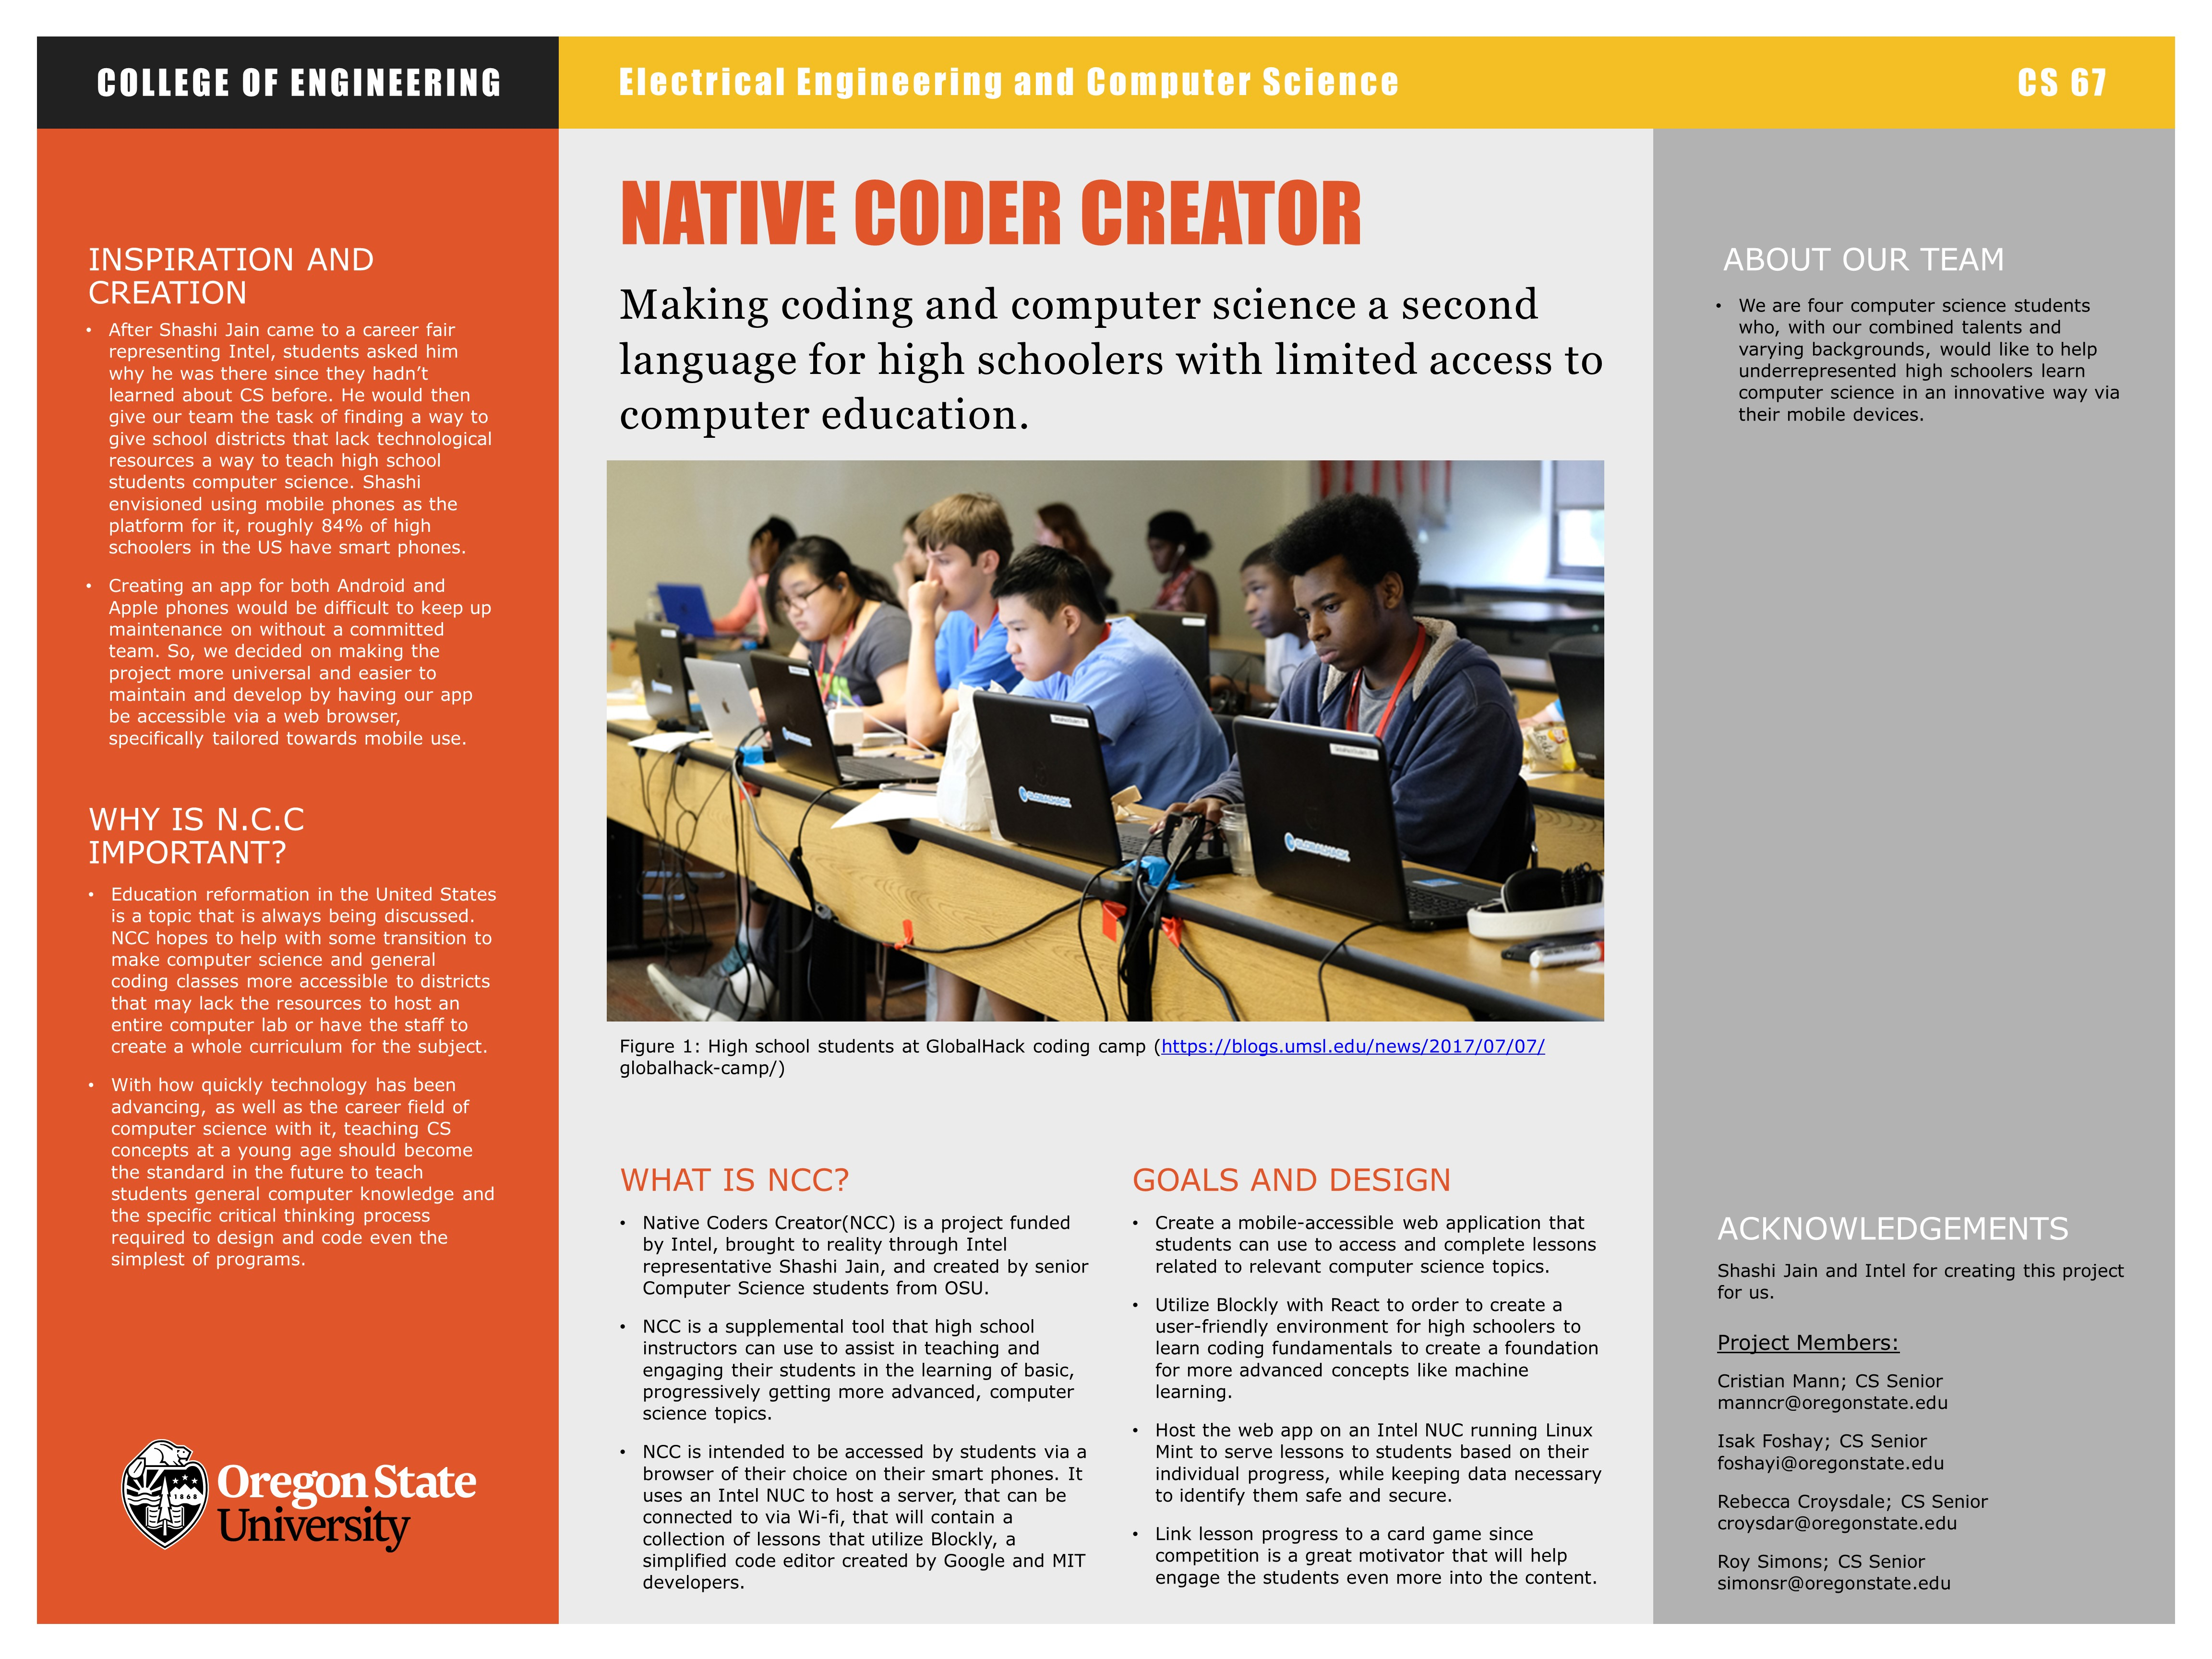
\includegraphics[width=18cm]{capstone_poster.jpg}
            \caption{Final Poster}
            \label{fig:2}
        \end{figure}

\clearpage
\section{Project documentation}
\subsection{Project structure and operation}
The application is served via an Intel NUC which creates a WiFi access point that the users can connect to. Once the students are connected to the WiFi they access the application via the web browser. Once the users are connected to the web browser they must register an account. Their information gets stored locally in the database and their passwords get hashed as a security measure. When a user logs in, the provided information gets checked with the information that is stored in the database. If correct, the user gets access to the application. \newline

The lessons that are provided, as well as the newly created lessons, are stored locally; no internet connection is required to access the lessons. The lessons are completed by the student users with Google's Blockly, which is a block-based visual programming language. The answer the student turns in is graded by a grading script, which is also written with Google's Blockly. The grading script is written by the teacher user, which allows the teacher to grade their students answers in their own custom way. The progress of the students are stored locally within their account. The only user that has access to all users progress is the teacher.\newline

%maybe add an in dept description of what happened when a student picks a lesson, completes a lesson and presses the grade button.

\subsection{How to install and run}
\subsubsection{Requirements}
To work with this project you will need Node.js version 13.8.x. The required operating system is Linux.
\subsubsection{Installation}
If you want to work with the application from your local machine, you first clone the repository from the project GitHub by doing git clone https://github.com/foshay/programming-for-kids.git .
Next, you run the setup.sh file in the setup directory, this installs all dependencies. Finally you run the start.sh file in the main directory to start the application. 
\subsubsection{Usage}
All users are required to be logged-in to get access to the application. Student users can just register their account to get full access to the student part of the application. There is one extra step for teacher user to get full access to the the teacher part of the application: they have use a one time password to register their account. This one time password is obtained by using the Google authenticator app to scan the QR code which is found in our GitHub in the "otp-qr.png" file.

\clearpage
\section{Recommended Technical Resources for Learning More}
%What web sites were helpful?% (Listed in order of helpfulness.)
%What, if any, reference books really helped?
%Were there any people on campus that were really helpful?
\begin{itemize}
    \item Blockly guide - https://developers.google.com/blockly
    \item ReactJS guide - https://reactjs.org/
    \item BlueprintJS UI toolkit - https://blueprintjs.com/docs/
    \item Sqlite3 database - https://www.sqlite.org/version3.html
\end{itemize}

\clearpage
\section{Conclusions and reflections}
\subsection{Isak Foshay Conclusions and reflections}
\begin{itemize}
    \item What technical information did you learn?
    \begin{itemize}
        \item I learned an immense amount of Javascript, Node.js, automating things with bash scripts, and REST API calls.
    \end{itemize}
    \item What non-technical information did you learn?
    \begin{itemize}
        \item I learned that putting lots of work into a project can be worth it in the end once you have a project you are happy with.
    \end{itemize}
    \item What have you learned about project work?
    \begin{itemize}
        \item Project work takes time and can seem grueling when no visible progress is being made.
    \end{itemize}
    \item What have you learned about project management?
    \begin{itemize}
        \item People respond well to being able to see what needs to be done (for example GitHub issues) in front of them. Different people work well with different things and project managers should focus on assigning tasks to people based on what they enjoy / are good at.
    \end{itemize}
    \item What have you learned about working in teams?
    \begin{itemize}
        \item Communication is key. Weekly meetings are a must as well as a record to keep track of what has been talked about in each meeting.
    \end{itemize}
    \item If you could do it all over, what would you do differently?
    \begin{itemize}
        \item I would make GitHub issues day 1 of coding. I would also record all of our meetings in order to have the transcripts for later documentation.
    \end{itemize}
\end{itemize}

\subsection{Rebecca Croysdale Conclusions and reflections}
\begin{itemize}
    \item What technical information did you learn?
    \begin{itemize}
        \item I learned a lot about API calls and sqlite. I was already proficient at react and JavaScript, which is why part of why we chose to work with those.
    \end{itemize}
    \item What non-technical information did you learn?
    \begin{itemize}
        \item  I learned how to be more assertive about making sure a client understands what is realistic.
    \end{itemize}
    \item What have you learned about project work?
    \begin{itemize}
        \item It is important to have set tasks for people to do and to assign those tasks to people. This ensures that people know that they are not doing the same work as another person. Having a definitive list of goals is also motivating.
    \end{itemize}
    \item What have you learned about project management?
    \begin{itemize}
        \item It is important to have someone take a leadership/organizing role. At other colleges, including PSU, this role is assigned after an interview process of the interested students. In our group, Isak assigned himself that role and did a fantastic job.
    \end{itemize}
    \item What have you learned about working in teams?
    \begin{itemize}
        \item Communication is important. Most of the time we had a problem, it was due to a miscommunication.
    \end{itemize}
    \item If you could do it all over, what would you do differently?
    \begin{itemize}
        \item I think we should have put more effort into contacting the client after he didn't show up to meetings. We did change the meeting time to fit into his schedule, but in hind sight, a quick text when he was late to meetings would have been beneficial.
        I learned that other teams were having meetings with their clients less often, and only when there was something specific to talk about. This may have worked better than weekly meetings.
        I also think we should have met up in person as a team to code more often, because each time we did, we got a lot of work done.
        
    \end{itemize}
\end{itemize}

\subsection{Cristian Mann Conclusions and reflections}
\begin{itemize}
    \item What technical information did you learn?
        \begin{itemize}
            \item How to create and interact with a database, a deeper understanding of JavaScript, how to protect a database's information, and how to handle authorization and authenticity when it comes to handles user accounts and access to certain information or pages.
        \end{itemize}
    \item What non-technical information did you learn?
        \begin{itemize}
            \item How to create a productive workflow using Github and how working alongside other people in person greatly increases productivity for all parties involved.
        \end{itemize}
    \item What have you learned about project work?
        \begin{itemize}
            \item Communication, from both client and team members, is essential. Also, that most your time will be spent researching/designing and trying to make things work more than actual coding, and that code created does not reflect work put into the design, research, and testing of that code.
        \end{itemize}
    \item What have you learned about project management?
        \begin{itemize}
            \item Splitting up the work early on and very well defining the tasks necessary for an issue to be deemed complete will make it easier to handle working on parts of a big project.
        \end{itemize}
    \item What have you learned about working in teams?
        \begin{itemize}
            \item The clashing of work styles and lack of communication really slows down development and can lead to conflict. 
        \end{itemize}
    \item If you could do it all over, what would you do differently?
        \begin{itemize}
            \item Show up to more meetings and not be afraid to say my ideas, opinions, and thoughts on others' ideas and opinions in relation to the project.
        \end{itemize}
\end{itemize}
\subsection{Roy Simons Conclusions and reflections}
\begin{itemize}
    \item What technical information did you learn?
    \begin{itemize}
        \item I learned to work with ReactJS, improved my JavaScript knowledge, found some great open source tools that can improve a user interface in an easier way than creating it all yourself.
    \end{itemize}
    \item What non-technical information did you learn?
    \begin{itemize}
        \item I learned that good communication with teammates and client is very important. I also learned that it is better to ask for help early, instead of trying to slowly figure it out yourself.
    \end{itemize}
    \item What have you learned about project work?
    \begin{itemize}
        \item Create structure and roles, I myself like to know clearly what I need to, what results are expected from me, what I can expect of others, and by when things are expected to be done.
    \end{itemize}
    \item What have you learned about project management?
    \begin{itemize}
        \item It is good to ensure that people know what they need to do, and by what time they are expected to be done with it. If someone is behind, it can hold up others in their progress. To have good project management good communication is key, and setting deadlines for certain features to be done.
    \end{itemize}
    \item What have you learned about working in teams?
    \begin{itemize}
        \item It can be difficult to work with people with different styles than yourself, but as long as the deadlines are met there are no real issues.
    \end{itemize}
    \item If you could do it all over, what would you do differently?
    \begin{itemize}
        \item I would start learning ReactJS already in fall, so that I could start working with the project from start of the development term. Second, I would have wanted to meet up more with our group, because the times we did meet up it was very productive.
    \end{itemize}
\end{itemize}

\clearpage

\section{Appendix 1}% Essential Code Listings}.You don't have to include absolutely everything, but if someone wants to understand your project, there should be enough here to learn from. If you worked within a larger project, something like a patch file might be a good way to go.
\emph{The files are too large to show here, so the paths to them from the Github repo are given, with "<root>" being the top directory that contains the README.md file.}
\subsection{React Routing}
\begin{lstlisting}
PATH: <root>/client/src/App/App.js
\end{lstlisting}
\underline{Description:} \\
The code in the file handles the routes the React server sends a user to upon any GET request to it. In here is where JSON web tokens (JWT) are checked to see if the user is allowed past the login or registration screens. Then, it checks if the user has access to the Teacher view or Student view, redirecting them according to the payload of the JWT.\\

\subsection{Blockly Composition}
\begin{lstlisting}
PATH: <root>/client/src/Blockly_comps/BlocklyComp.js
\end{lstlisting}
\underline{Description:} \\
The Blockly environment used in lesson creation, lesson editing, student lesson completion, and viewing of a student's solution to a lesson are created with this file of code. \\

\subsection{Registration}
\begin{lstlisting}
PATH: <root>/client/src/Screens/LoginRegister/RegisterForm.js
\end{lstlisting}
The student and teacher registration forms are derived from the React component within this file. Here, the majority of the page will be served, including the one-time password field if it's a teacher, as well as checking that password's validity. It will also check that a username and password fit the minimum requirements and that the confirmation password matches, giving feedback accordingly. After receiving a valid input, the appropriate handler for the type of user will be called, sending a request to the API server to register the account if it is valid, relaying the success or failure of the registration request to the user. 

\clearpage
\section{Appendix 2}% Anything else you want to include. Photos, etc.
\begin{figure}[h]
    \centering
    
\includegraphics[width=\textwidth]{caps1}
    \caption{Start screen.}
    %\label{fig:mesh1}
\end{figure}

\begin{figure}[h]
    \centering
    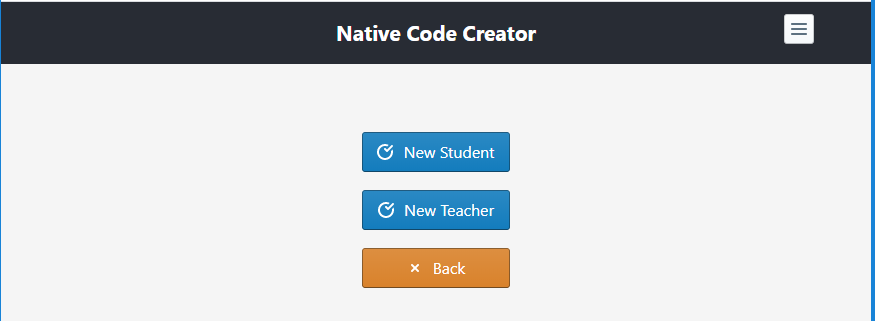
\includegraphics[width=\textwidth]{caps2}
    \caption{Register choice screen.}
    %\label{fig:mesh1}
\end{figure}

\begin{figure}[h]
    \centering
    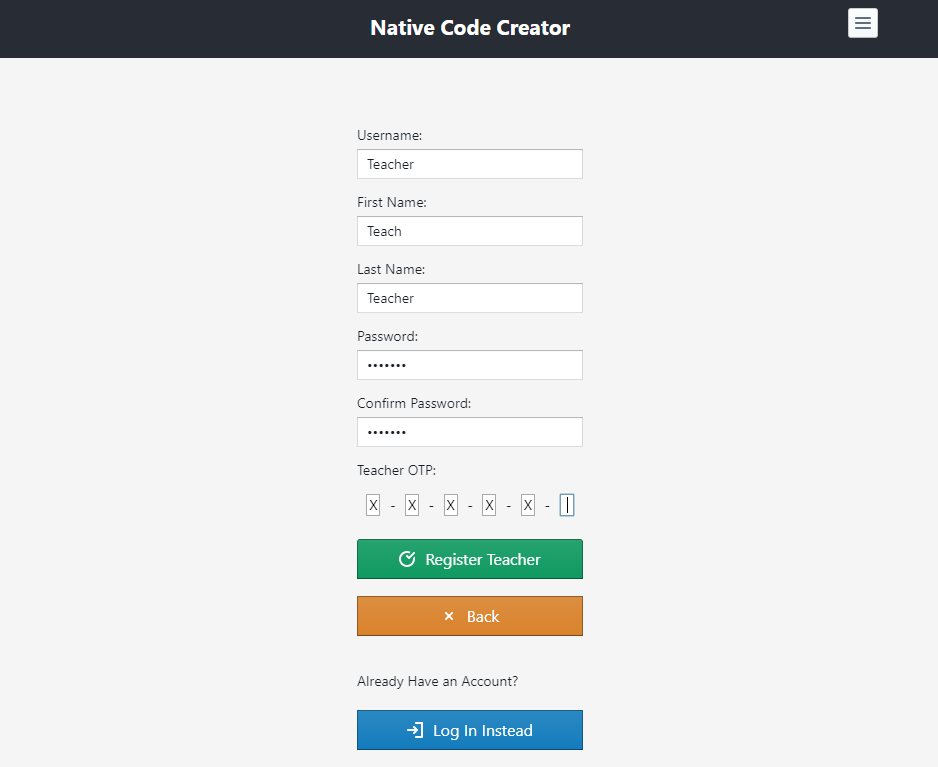
\includegraphics[width=\textwidth]{caps3}
    \caption{Register screen for teachers.}
    %\label{fig:mesh1}
\end{figure}

\begin{figure}[h]
    \centering
    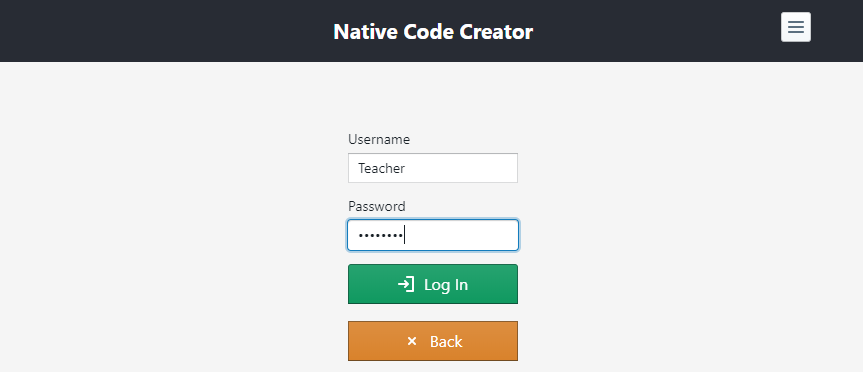
\includegraphics[width=\textwidth]{caps4}
    \caption{4. Log-in screen.}
    %\label{fig:mesh1}
\end{figure}

\begin{figure}[h]
    \centering
    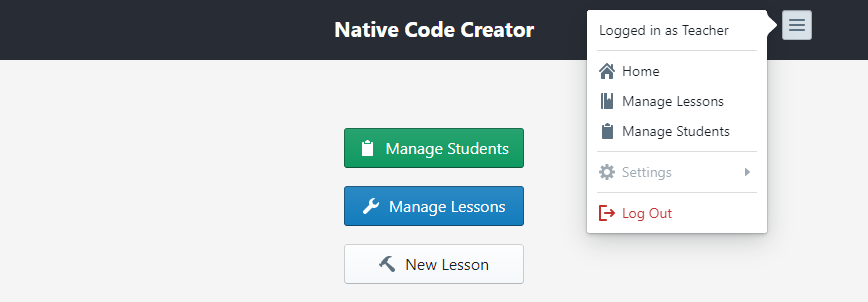
\includegraphics[width=\textwidth]{caps5}
    \caption{The home screen for teacher users.}
    %\label{fig:mesh1}
\end{figure}

\begin{figure}[h]
    \centering
    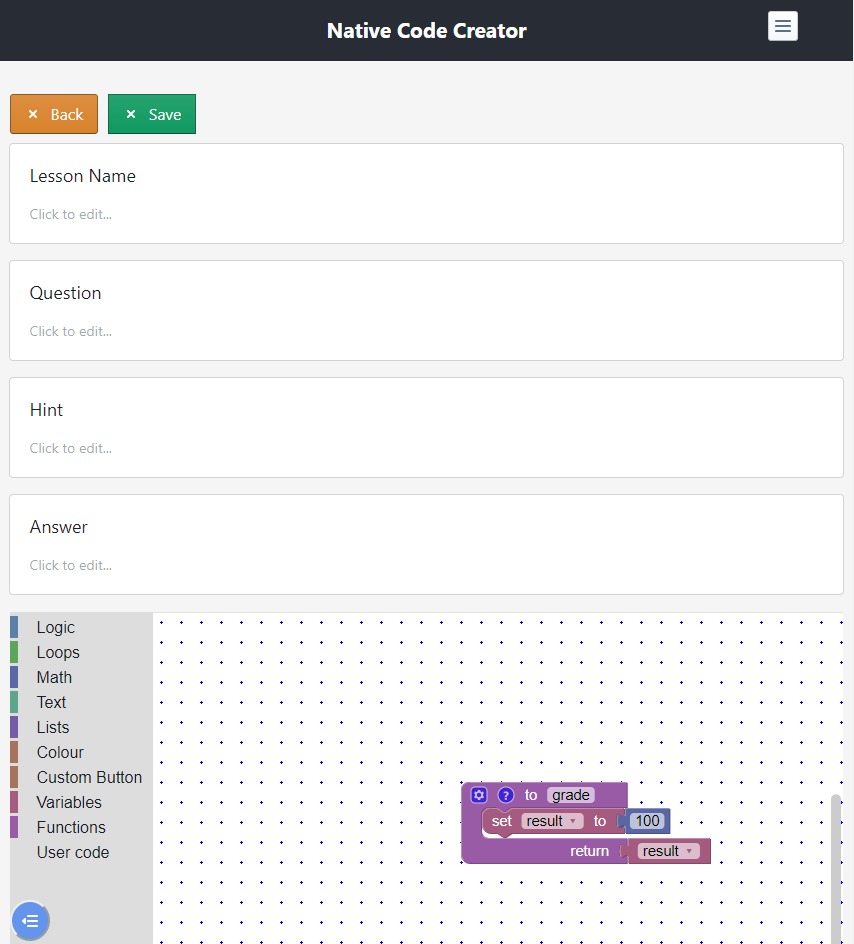
\includegraphics[width=\textwidth]{caps6}
    \caption{Create new lesson screen.}
    %\label{fig:mesh1}
\end{figure}

\begin{figure}[h]
    \centering
    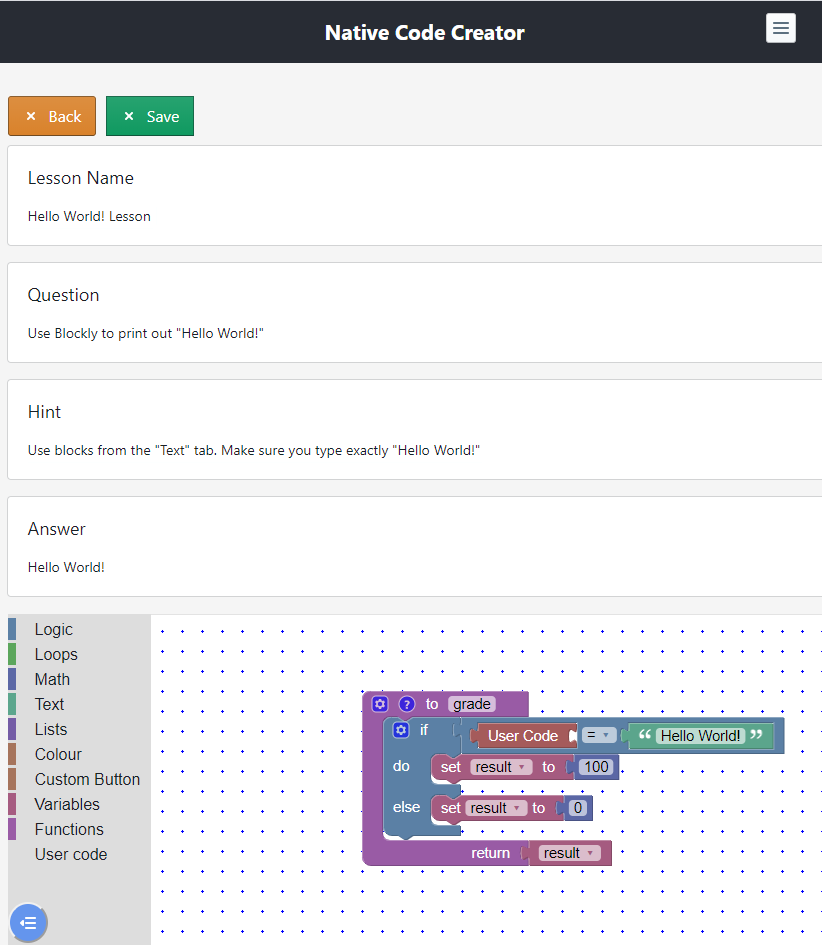
\includegraphics[width=\textwidth]{caps7}
    \caption{Filled out lesson screen, that will grade the " Hello World!" lesson.}
    %\label{fig:mesh1}
\end{figure}

\begin{figure}[h]
    \centering
    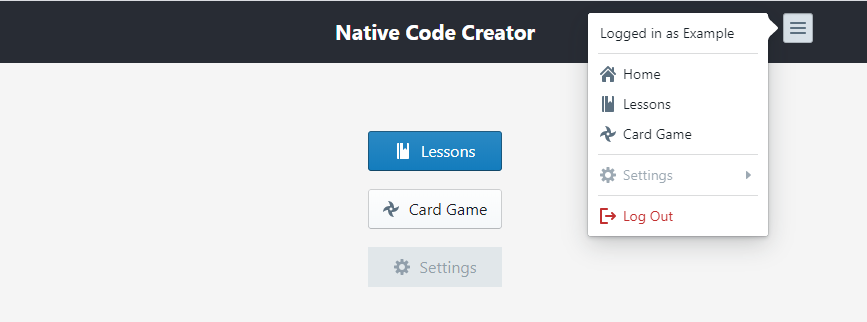
\includegraphics[width=\textwidth]{caps8}
    \caption{The home screen for student users.}
    %\label{fig:mesh1}
\end{figure}

\begin{figure}[h]
    \centering
    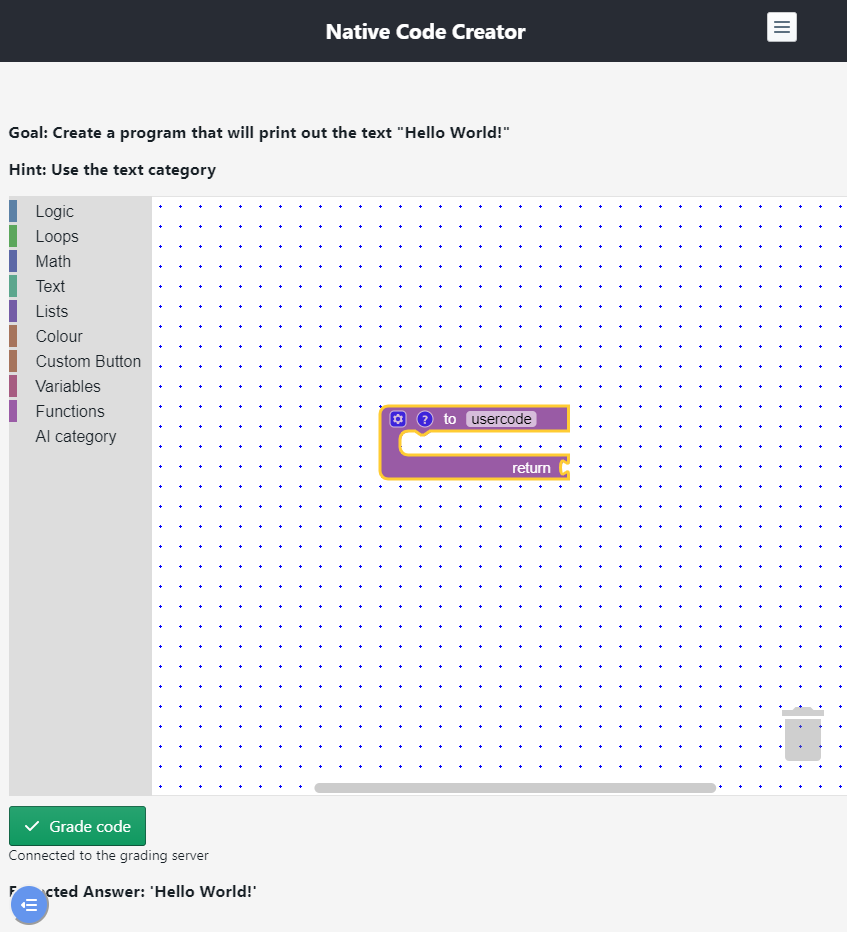
\includegraphics[width=\textwidth]{caps9}
    \caption{The "Hello World!" lesson for the student users.}
    %\label{fig:mesh1}
\end{figure}

\begin{figure}[h]
    \centering
    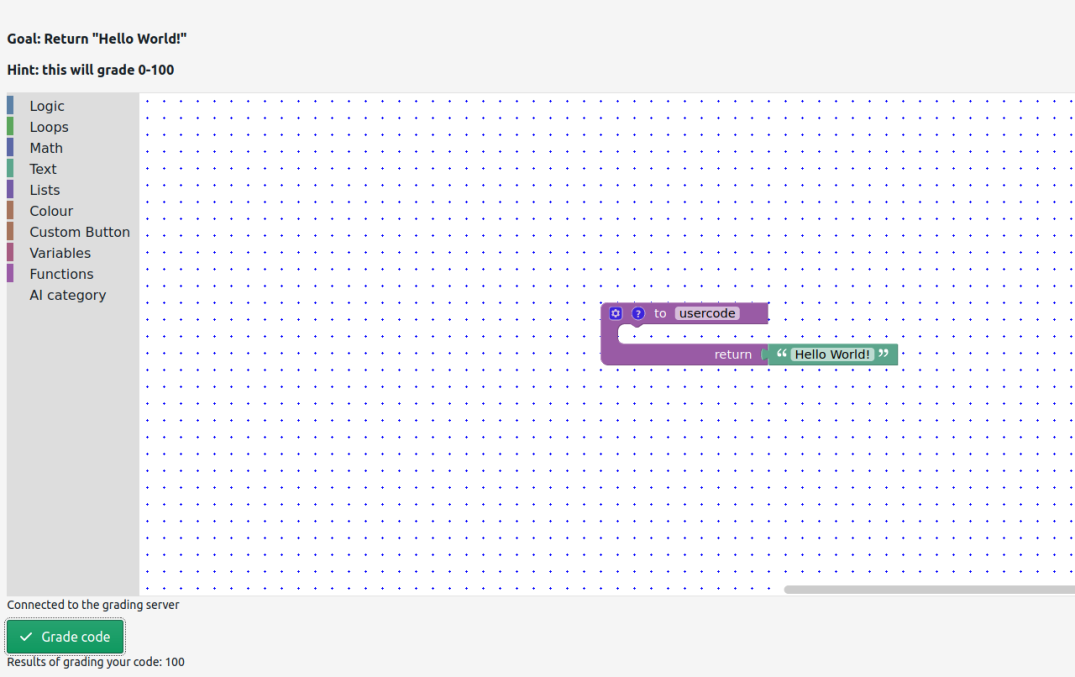
\includegraphics[width=\textwidth]{caps10}
    \caption{The "Hello World!" lesson answered correctly, resulting into 100 points.}
    %\label{fig:mesh1}
\end{figure}

\begin{figure}[h]
    \centering
    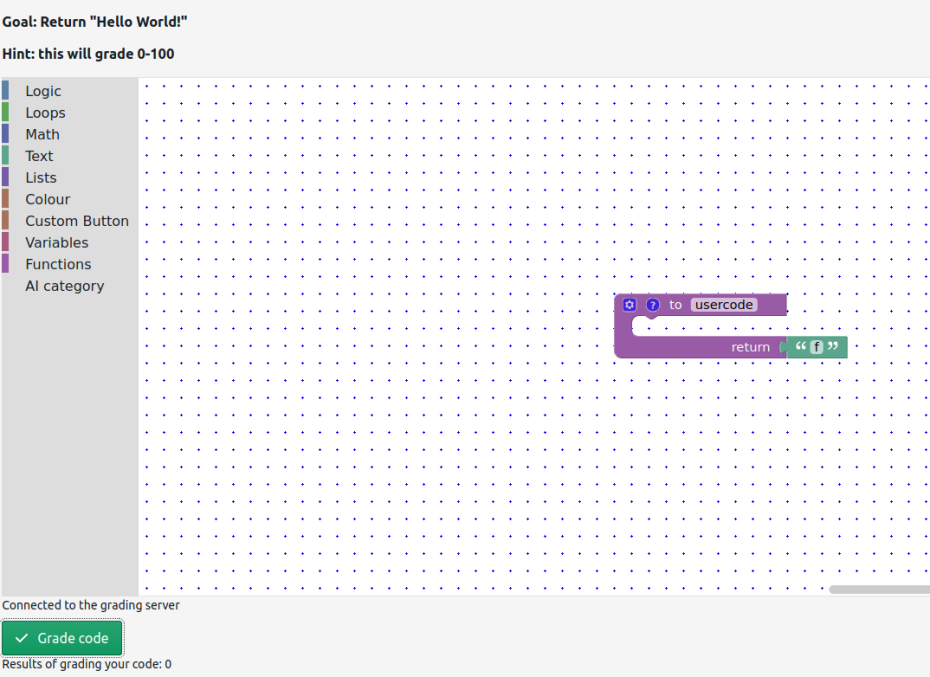
\includegraphics[width=\textwidth]{caps11}
    \caption{The "Hello World!" lesson answered incorrectly, resulting into 0 points.}
    %\label{fig:mesh1}
\end{figure}

\clearpage
\section{Appendix 3}%: Include the criticisms from the code review and your responses to each criticism in an appendix in your final project archive documentation
\subsection{Build}
The build was smooth for anyone on Linux (our project's intended OS)
\subsection{Legibility}
\paragraph{Could you add header comments for functions to explain how the function interacts with the project as a whole?}
This has not been done yet. Currently, we have comments for what the functions do, and going through all of our many functions will take time.
\paragraph{Could you delete commented out code?}
Yes, we will be doing that in our final PRs for code freeze.
\subsection{Implementation}
\paragraph{Could you separate database calls to a different library?}
This is something that could be done but has not.
\subsection{Maintainability}
\paragraph{No unit tests.}
Because this is a web-based project unit tests are difficult. Currently, we still have no unit tests
\subsection{Requirements}
\paragraph{Where is the requirements document?}
Our project had changed substantially throughout the year and did not reflect what our project ended up being. We have now updated the requirements document. (Currently found here: \href{https://github.com/foshay/programming-for-kids/wiki/Requirements_2_0.pdf}{<Requirements Document Link>})
\subsection{Other}
\paragraph{Will placeholders like the card game remain?}
No. We talked with our client and the lessons were more important to him than the card game.
\paragraph{Will grade tracking be added?}
Yes. There is now a page for grade tracking that teachers can navigate to.
\paragraph{Will python code be sandboxed?}
Not for code freeze. Security was one of the lowest priorities for our client so we did not focus on this aspect of the project.

\end{document}
